%=========================================================================
% (c) Michal Bidlo, Bohuslav Křena, 2008

\chapter{Úvod}
Linux je slobodný open source operačný systém obľúbený vďaka výbornej podpore ľudí z~komunity, možnosti modifikovania zdrojových kódov a v~neposlednom rade širokého spektra dostupného bezplatného softvéru. Vďaka týmto, ale aj mnohým iným vlastnostiam a~výhodám  ho môžeme nájsť na~väčšine superpočítačoch a~serveroch.

Častokrát sú tieto servery spájané do~väčších celkov a~vytvárajú serverové clustery a~tie zasa serverové farmy. K~takejto agregácií dochádza z~viacerých dôvodov, napríklad pre~zaistenie dostupnosti služby, zvýšenie výpočtového výkonu a~podobne. Takýto cluster môže obsahovať desiatky až~stovky serverov, pričom treba zaistiť ich bezproblémový chod. \\ Každé z~týchto zariadení obsahuje určité požiadavky, a~teda môže byť rôzne zaťažené prípadne sa na~ňom môže vyskytnúť porucha alebo môže byť taktiež cieľom útočníkov. Preto je nevyhnutné mať pod dohľadom každý uzol, monitorovať jednotlivé operácie, ktoré spracováva pre~optimálne rozloženie zaťaženia medzi jednotlivé uzly clusteru, predvídať poddimenzovanosť uzlov z~hľadiska výkonu a~detekovať možné problémy zavčas, ešte pred koncovým užívateľom. V~závislosti na~počte serverov sú používané rôzne techniky monitorovania. V~prípade malých počtov serverov systémový administrátor využíva vlastné vzájomne nezávislé skripty, no v~prípade serverových fariem sa používajú zväčša monitorovacie nástroje ako Nagios, Zabbix a~im podobné programy.

Táto bakalárska práca vznikla z~dôvodu skombinovania výhod oboch prístupov monitorovania systému s~ohľadom na~využitie už existujúcich skriptov s~ich minimálnou \mbox{modifikáciu}. Výsledný monitorovací program bude rozdelený do~menších skriptov, ktoré budú môcť byť použité aj samostatne. Tento prístup je zvolený z~dôvodu modularity a~flexibility výsledného nástroja

V~nasledujúcej kapitole \ref{teoria} je opísaná motivácia použitia operačných systémov, v~skratke je opísaný systém GNU/Linux a~teória k~počítačovému clusteru. V~ďalšej kapitole \ref{monitorovanie} pojednávajúcej o~monitorovaní sa bližšie pozrieme na~používané monitorovacie nástroje Nagios a~Zabbix a~protokol syslog. V~kapitole \ref{navrh} si popíšeme návrh monitorovacieho nástroja s~opisom jeho kľúčových vlastností, hierarchického rozdelenia skriptov a rozdielom oproti existujúcim riešeniam. Kapitole \ref{implementacia} sa pozrieme na zaujímavé prvky skriptov, formát notifikačnej správy a taktiež na implementáciu nasadzovacieho skriptu. Posledná kapitola \ref{testovanie} opisuje testovanie, a to predovšetkým testovacie prostredia a testovanie kľúčových prvkov programu.
  


\chapter{Teória}
\label{teoria}
\section{Operačný systém} 
Operačný systém je základom pre~každý výpočtový systém. Je to počítačový program, ktorý vytvára spojujúcu medzivrstvu medzi hardvérom, užívateľmi a~ich užívateľským softvérom. Medzi hlavné role operačných systémov patrí správa prostriedkov a~taktiež zabezpečenie prostredia užívateľom pre~bezproblémový prístup k~užívateľským programom. Operačný systém by mal spravovať prostriedky s~ohľadom na~efektivitu a~bezpečnosť. Prostriedky umožňuje spravodlivo rozdeľovať medzi užívateľov, užívateľský softvér a~teda dáva možnosť viacerým procesom zdieľať rovnaký procesor, priestor vo volatilných a~nevolatilných~pamätiach. Druhá zmienená rola je veľmi dôležitá a~k~jej zaisteniu je nutné jednotné rozhranie, ktoré zabezpečuje prenositeľnosť jednotlivých užívateľských aplikácií. Operačný systém poskytuje používateľom abstrakciu a~teda pre~užívateľa zakrýva nízkoúrovňové operácie. \cite{ios}

Presná definícia, čo všetko je súčasťou operačného systému nie je jednotná, niekedy sa tým myslí iba jadro, inokedy okrem jadra tiež grafické alebo textové rozhranie, systémové aplikačné programy a~ovládače.
\section{Jadro OS}
Jadro operačného systému nazývané tiež kernel je najnižšia a~najzákladnejšia časť operačného systému. Kernel sa zavádza ako prvý a~beží počas celej doby chodu operačného systému, pričom je uložený v~operačnej pamäti a~podľa potrieb spúšťa ostatné súčasti operačného systému. Pre užívateľa a~užívateľský softvér kompletne zapuzdruje hardvér tým, že na~neho priamo naväzuje. Zariaďuje základnú správu prostriedkov a~to prevažne správu kontextu a~nastavenie hardvéru. Tým, že obvykle beží v~privilegovanom režime, tak má neobmedzený prístup k~hardvéru a~môže nad ním vykonávať rôzne operácie. Počet služieb, ktoré jadro poskytuje zväčša závisí na~kompromise medzi viacerými faktormi a~to hlavne bezpečnosťou, efektivitou a~flexibilitou. \cite{ios}
\section{Unix}
Unix je univerzálny, viacužívateľský, viacúlohový operačný systém vyvinutý v~70.\,--\,tých rokoch minulého storočia \cite{unix-root}. Tento operačný systém bol vyvinutý v~spoločnosti Bell Labs Kenom Thompsonom a~Dennisom Ritchiem \cite{unix-root}. Ide o~prvý prenositeľný operačný systém, pričom tejto vlastnosti vďačí programovaciemu jazyku C, do~ktorého bol po~čase prepísaný a~ktorého tvorcom je Dennis Ritchie. Vďaka tomu ho bolo možné takmer od počiatku použiť na~širokej škále zariadení resp. platforiem a~predurčilo ho k~ďalšiemu úspechu. Unix je veľmi obľúbený v~akademickej sfére hlavne z~dôvodu otvoreného kódu, bezplatnosti a~spoľahlivosti.
\\\\
\noindent Výhody Unix-u:
\begin{itemize}
	\item flexibilita\,--\,môže byť inštalovaný od vstavaných zariadení až~po~superpočítače.  
	\item stabilita\,--\,oproti mnohým iným operačným systémom je prevádzkyschopný s~dostatočným výkonom napriek absencii reštartu v~porovnaní s~MS Windows.
	\item bezpečnosť\,--\,pokročilé nastavenie prístupových práv a~SELinux.
	\item bezplatnosť\,--\,minimalizuje počiatočné náklady za licencie.
	\item open-source\,--\,každý môže nahliadnuť do~zdrojových kódov a~modifikovať ich.
\end{itemize} 

\noindent Od vzniku Unix-u bolo uvedených mnoho derivátov, ako napríklad \cite{unix-based}:
\begin{itemize}
	\item BSD
	\item Solaris
	\item GNU/Linux
	\item macOS
\end{itemize}
\section{GNU/Linux}
GNU je operačný systém inšpirovaný UNIX-om patriaci do~skupiny UNIX-like OS, ktorého vývoj započal v~roku 1984  Richardom Stallmanom na~MIT. Myšlienka a~filozofia tohto operačného systému je sloboda užívateľov spúšťať, kopírovať, distribuovať, študovať a~vylepšovať softvér. Motiváciou bolo vytvoriť operačný systém z~čisto slobodného~\mbox{softvéru}. Operačný systém GNU využíva jadro Linux, ktoré bolo spočiatku vyvíjané fínskym študentom Linusom Torvaldsom a~nahradilo jadro Hurd vyvíjané projektom GNU. \cite{gnu}

V~súčasnosti je GNU/Linux vyvíjaný za pomoci komunity vývojárov, v~ktorej sú jednotlivci, ako aj veľké korporácie z~celého sveta, napríklad \mbox{Red Hat}, Intel, IBM, SUSE \cite{gnu}.

Operačný systém GNU/Linux je vyvíjaný s~ohľadom na~podporu väčšiny softvéru vyvinutého pre~Unix. Medzi najznámejšie patria Bourne shell, systém X Window, mkfs, fsck a~mnohé ďalšie.

Od svojho vzniku si GNU/Linux udržuje rastúce tempo v~podiele zastúpenia operačných systémov. Bezkonkurenčne vedie v~percentuálnom nasadení na~superpočítačoch \cite{marketsharesupercomputers}, kde ostatné operačné systémy sú v~minoritnom zastúpení. Taktiež má výrazný náskok v~oblasti webových serverov \cite{marketshareservers}, no jeho podiel na~osobných počítačoch alebo pracovných staniciach je okolo 5\%.

\section{Distribúcie}
Linuxová distribúcia je operačný systém pozostávajúci z~kolekcie softvérového vybavenia a~správcu balíkov založený na~Linuxovom jadre \cite{linux-distros}. Pred inštaláciou samotného operačného systému by sme si mali vybrať vhodnú distribúciu pre~dané zariadenie z~hľadiska nárokov na~hardvér, počtu súčastí distribúcie, podpory zo strany komunity a~prostredia nasadenia.

Distribúcie môžu byť ihneď pripravené k~použitiu a~to napríklad spustením z~USB kľúča, nainštalovaním na~pevný disk alebo sú distribuované ako zdrojový kód a~je ich nutné skompilovať.

Primárne sa distribúcie rozdeľujú podľa prostredia nasadenia a~to na~distribúcie určené pre~osobné počítače, pracovné stanice a~tie, ktoré sú určené pre~nasadenie na~serveroch \cite{linux-distros}. Ich hlavným rozdielom je množstvo zabraného miesta na~disku, prítomnosť grafického užívateľského rozhrania a~počtu obsiahnutých balíkov. Distribúcie určené pre~serveri sú zväčša zamerané na~výkon a~teda typicky neobsahujú grafické užívateľské rozhranie a~obsahujú iba to najnutnejšie, pričom všetky potrebné balíčky je možné dodatočne doinštalovať. \mbox{Pokročilí}~užívatelia a~administrátori si môžu vytvoriť vlastnú distribúciu, ktorá bude zahŕňať kľúčové balíčky a~súčasti operačného systému pre~konkrétne nasadenie, čím sa zvýši efektivita a~zároveň bude hardvér menej zaťažený.
\\\\
\noindent Populárne distribúcie pre~PC/Workstation:
\begin{itemize}
	\item Ubuntu
	\item Debian
	\item Fedora
	\item Arch
	\item Mint
\end{itemize}
\noindent Populárne distribúcie pre~serverové nasadenie:
\begin{itemize}
	\item Red Hat Enterprise Linux
	\item Ubuntu Server
	\item Centos
	\item SUSE Enterprise Linux
	\item Debian
\end{itemize}
\section{Cluster}
Požiadavky na~výkon počítačov neustále stúpajú, preto je nevyhnutnosťou namiesto jedného serveru, ktorý by náročné úlohy a~záťaž nezvládal, zoskupiť viacero počítačov a~tým urýchliť výpočtové operácie. Práve tento dôvod viedol k~vytvoreniu počítačového clusteru. 


Počítačový cluster je zoskupenie aspoň dvoch počítačov (uzlov), ktoré spolu spolupracujú a~navonok sa tvária ako jeden počítač \cite{cluster-book}. Dôvody pre~nasadenie takéhoto riešenia sú rôzne, pričom zväčša ide o~navýšenie výpočtového výkonu, zvýšenie spoľahlivosti a~prerozdeľovanie záťaže.
\\\\
\begin{figure}[H]
	\begin{center}
		\scalebox{0.5}{\includegraphics{obrazky-figures/ha_cluster.jpg}}
		\caption{Cluster s~vysokou dostupnosťou \cite{cluster-web}}
		\label{cluster}
	\end{center}
\end{figure}

\begin{figure}[H]
	\begin{center}
		\scalebox{0.4}{\includegraphics{obrazky-figures/active_active_cluster.jpg}}
		\caption{Active-Active Cluster \cite{cluster-web}}
		\label{cluster}
	\end{center}
\end{figure}

\begin{figure}[H]
	\begin{center}
		\scalebox{0.6}{\includegraphics{obrazky-figures/active_passive_cluster.jpg}}
		\caption{Active-Passive Cluster \cite{cluster-web}}
		\label{cluster}
	\end{center}
\end{figure}

\subsection*{Typy clusterov}
Z~hľadiska miesta nasadenia a~zverených úloh pre~výpočet a~role sú počítačové clustery rozdelené do~viacerých kategórií. V~závislosti na~použitom operačnom systéme sú častými zástupcami Windows cluster a~Linux cluster.
\\\\
\noindent Typy clusterov \cite{cluster-book}:
\begin{itemize}
	\item Cluster s~vysokou dostupnosťou
	\item Cluster s~rozložením záťaže
	\item Výpočtový cluster
	\item Úložný cluster
\end{itemize}
\subsubsection*{Cluster s~vysokou dostupnosťou}
Po určitej dobe prevádzky hardvér počítača degraduje, preto je nutné počítať s~výpadkom služieb bežiacich na~serveri. Z~tohto dôvodu vznikol cluster s~vysokou dostupnosťou alebo inak nazývaný High availability cluster. V~prípade výpadku služby na~niektorom z~uzlov, preberie iný uzol, ktorý poskytuje tú istú službu jeho rolu. Tým je zaistená dostupnosť služby. Tento koncept taktiež umožňuje vykonávať plánovaný servis bez toho, aby zákazník pocítil výpadok alebo zníženie výkonu. \cite{cluster-book}

\subsubsection{Cluster s~rozložením záťaže}
Tento typ clusteru využíva metódu, kedy sú dáta distribuované medzi dvoma a~viac servermi, pričom dáta na~všetkých serveroch by mali byť totožné. \mbox{Počíta}~sa s~ideálnym rozložením záťaže pre~jednotlivé uzly. Typicky je tento typ clusterov často používaný pre~web servery, kde zaisťuje vysokú rýchlosť a~zároveň garanciu dostupnosti kvôli redundancii. V~prípade dvoch serverov vytvárajúcich tento typ clusteru, je jeden určený za primárny a~ďalší za sekundárny, pričom záťaž medzi tieto dva uzly rozdeľuje tzv. Master load balancer. Jednou z~nevýhod tohto typu clusteru je nutnosť replikácie dát a~teda redundancie, čo sťažuje prácu pre~zaistenie konzistencie dát uložených na~oboch uzloch a~taktiež niekoľkonásobné finančné zaťaženie v~závislosti na~počte uzlov. \cite{cluster-book}

\subsubsection*{Výpočtový cluster} Výpočtový cluster využíva sa na~náročné výpočty, kde by jeden vysokovýkonný počítač bol priveľmi drahý. Takýto cluster sa skladá z~aspoň dvoch počítačov pričom nemusia byť veľmi výkonné, no sú navzájom prepojené vysokorýchlostnou sieťou a~zdieľajú medzi sebou výpočtové zdroje. \cite{cluster-book}

\subsubsection{Úložný cluster}
 Tento cluster patrí k~špeciálnym typom clusteru s~rozložením záťaže, ktorý zaisťuje  prístup k~diskovej kapacite rozdelenej medzi viacero počítačov kvôli vyššej prenosovej rýchlosti a~zaisteniu spoľahlivosti. Používa špeciálny súborový systém, ktorého príkladom je GFS od spoločnosti \mbox{Red Hat} zaisťujúci redundanciu, konzistenciu, integritu dát, mechanizmus zamykania súborov a~pokrytie výpadkov. \cite{cluster-book} 

\subsection*{Nevyhnutné prvky na vytvorenie clusteru}
Počítačový cluster vzniká vtedy, ak sú vzájomne prepojené aspoň dva počítače, ideálne pre~zaistenie dostupnosti a~vyváženého výkonu je však odporúčané použiť viacej uzlov. \mbox{Druhým}~predpokladom je prepojenie počítačov vysokorýchlostnou počítačovou sieťou, ktorá zabezpečí vysoký tok dát a~to najmä pri~implementácií webového clusteru s~rozložením~\mbox{záťaže}. Posledným krokom je voľba správcu zdrojov clusteru, ktorý sa postará o~prerozdeľovanie záťaže, nakonfigurovanie jednej spoločnej IP adresy pre~uzly v~clusteri a~vykoná ďalšie nastavenia potrebné pre~prevádzku. \cite{cluster-book}

\subsection*{Správcovia zdrojov clusterov}
Každý uzol clusteru musí byť spravovaný nejakým programom, ktorý zaistí migráciu služby na~iný uzol v~prípade poruchy alebo zvýšeného dopytu po~službe, prípadne riadenie \mbox{rozloženia} \mbox{záťaže}. Tento softvér sa nazýva správca zdrojov clusteru. Príkladmi takéhoto softvéru sú Pacemaker, oneSIS, OpenHPC, Linux-HA.

\section{Python}
Programovací jazyk \mbox{Python} je interpretovaný, interaktívny, objektovo orientovaný programovací jazyk vytvorený holanďanom Guidom van Rossom \cite{python}. Jeho veľkou výhodou je možnosť využitia na~širokom spektre operačných systémov a~taktiež fakt, že je vyvíjaný ako open source projekt.

Syntax \mbox{Python}u je jedným z~dôvodov, prečo sa stal tak populárnym. Je totiž navrhovaný s~ohľadom na~čitateľnosť a~syntax je veľmi podobná programovaciemu jazyku C. \mbox{Veľkým}~rozdielom oproti iným jazykom je spôsob zápisu blokov kódu, ktorý je daný odsadením a~nie ako v~jazyku C pomocou zátvoriek alebo v~Pascale kľúčovými slovami \texttt{Begin} a \texttt{End}.

V~súčasnosti sa na~tvorbu programov používajú dve verzie a~to \mbox{Python} 2.x a~\mbox{Python} 3.x. Aj keď by sa mohlo zdať, že ide o~ten istý programovací jazyk, niektoré syntaktické konštrukcie nie sú kompatibilné medzi oboma verziami \cite{python}. V~neprospech \mbox{Python} 3.x hovorí aj to, že mnohé knižnice sú určené pre~\mbox{Python} 2.x a~teda často úplne \mbox{nepoužiteľné}. \mbox{Nedávno}~zverejnené prehlásenie hovorí o~konci vývoja a~podpory \mbox{Python} 2.x, preto pre~budúce programy je výhodnejšie použiť \mbox{Python} 3.x\footnote[1]{http://legacy.\mbox{Python}.org/dev/peps/pep-0373/}.

\section{Nasadzovací softvér}
\label{nasadenie} 
Každý program, ktorý chceme používať je v~prvom rade nutné nainštalovať a~nakonfigurovať pre~správne fungovanie na~zariadení a~pre konkrétne použitie. Pri nasadení, teda inštalácií a~konfigurácií programu na~jednom zariadení nie je problém tieto kroky aplikovať manuálne, problémom však je nasadenie programu alebo programov na~desiatkach až~stovkách \mbox{zariadení}. Pre tento účel vznikli špecializované programy, ktoré zjednodušujú nasadenie aplikácií vo výpočtových centrách s~množstvami počítačov a~clusterov.

Nasadenie softvéru je súbor procesov alebo aktivít, ktoré vedú k~dostupnosti požadovaného inštalovaného softvéru \cite{deployment-web}. Špecializované programy a~knižnice programovacích jazykov umožňujú nielen samotné nasadenie, teda inštaláciu a~konfiguráciu programu, ale aj ďalšie dôležité aktivity medzi ktoré patrí aktualizácia, odinštalácia a~sledovanie nainštalovaných verzií \cite{deployment-web}. Je treba si uvedomiť, že tento softvér okrem uľahčenia práce znižuje riziko vzniku rôznych chýb pri~aktualizáciách a~nasadení. Dôležitou vlastnosťou je taktiež stránka bezpečnosti, ktorú napomáha zlepšovať spomínaným sledovaním verzií a~hromadnou aktualizáciou na~všetkých staniciach. Namiesto manuálnych aktualizácií, ktoré pri~desiatkach až~stovkách uzloch môžu nakopiť chyby a~zároveň sú časovo náročne, aktualizácia pomocou tohto softvéru je vykonávaná hromadne na~zvolených zariadeniach s~rovnakými podmienkami a~postupom.

Pridanou hodnotou nasadzovacieho softvéru je okrem ušetreného času taktiež zníženie nákladov a~rýchlejšia dostupnosť nasadzovanej služby v~kombinácií s~nižším rizikom vnesenia chýb.

Nasadzovacieho softvéru existuje celá rada, pričom sa líšia ich primárnym určením. Nástroje Travis a~Jenkins sú primárne určené na~automatizované testovanie, no zvládnu aj nasadenie otestovaných programov. Medzi ďalšie nástroje, respektíve knižnice určené na~nasadenie patria napríklad \mbox{Python} Fabric a~Capistrano. Najuniverzálnejšími a~veľmi mocnými nástrojmi na~nasadenie, konfiguráciu, aktualizáciu sú Ansible od firmy \mbox{Red Hat}, ale aj Puppet alebo Salt.

\section{Ansible}
Ansible je program na~automatizáciu nasadenia aplikácií a~správu konfigurácií \cite{ansible}. Jeho veľkou devízou je multiplatformnosť, je ho možné používať ako na~staniciach s~operačným systémom Linux, tak aj na~Microsoft Windows. Konfiguračný súbor tzv. Ansible \mbox{Playbook} je veľmi dobre čitateľný pre~používateľa aj stroj a~nevyžaduje špeciálne \mbox{programátorské nároky}. Ansible je napísaný v~programovacom jazyku \mbox{Python} pre~operačné systémy Linux a~v~PowerShell pre~operačný systém Windows \cite{ansible}.
\subsection*{Inštalácia}
Pre správu jednotlivých počítačov (uzlov) musíme nainštalovať na~tzv. kontrolný uzol, ktorým je počítač, z~ktorého bude prebiehať riadenie, program Ansible \cite{ansible}. Výhodou je, že na~žiaden spravovaný uzol nemusíme inštalovať agenta, ktorý by komunikoval a~bol riadený kontrolným uzlom, pretože na~systémoch GNU/Linux sa na~riadenie \mbox{použije SSH}. Tento dizajn zjednodušuje prvotné nasadenie samotného Ansible a~zvyšuje bezpečnosť, pretože neexistuje agent, ktorý by mohol byť napadnutý potenciálnym útočníkom.

\subsubsection*{Kľúčové prvky}
Na automatizovanie nasadenia, úloh a~správu je potrebných niekoľko kľúčových prvkov Ansible. Na obrázku \ref{ansible_scheme} môžeme vidieť architektúru Ansible spolu s~kľúčovými prvkami.

\begin{itemize}
	\item Ansible Playbook\,--\,využíva jazyk YAML a~definuje úlohy a~role pre~jednotlivé uzly.
	\item Inventory\,--\,zoznam uzlov, ktoré sú dostupné Ansiblu. Je to konfiguračný súbor obsahujúci IP adresu a~meno uzlu (hostname), ktorý môže byť riadený.
	\item Modules\,--\,jednotky, ktoré vykonávajú a~riadia danú úlohu, umožňujú inštaláciu, volania API a~prístup k~systémovým súborom. Moduly môžu byť napísané v~štandardných skriptovacích jazykoch, ako napríklad \mbox{Python}, Bash, Perl. 
\end{itemize}

\begin{figure}[H]
	\begin{center}
		\scalebox{0.5}{\includegraphics{obrazky-figures/ansible_scheme.png}}
		\caption{Architektúra Ansible \cite{ansible}}
		\label{ansible_scheme}
	\end{center}
\end{figure}

\subsubsection*{Ansible Playbook}
\label{ansible_playbook}
Príklad Ansible Playbook môžeme vidieť nižšie \ref{ansible_playbook_alg}. Súbor definujúci nasadenie je napísaný v~jazyku YAML a~vykonáva sa sekvenčne. Nižšie uvedený playbook obsahuje jeden play, tri úlohy (tasks) a~jeden handler. Na riadku číslo 2 definujeme skupinu zo zoznamu uzlov Inventory. Na riadkoch 3\,--\,5 deklarujeme premenné, s~ktorými \mbox{budeme pracovať}. \mbox{Nasledujú} úlohy (tasks), ktoré musia byť pomenované a~ďalej na~riadku 9 definujeme použitý modul, konkrétne yum a~čo má vykonať. Taktiež je možné použiť šablónu (template), ako na~riadku 11, ktorá obsahuje deklarácie premenných, ktoré prepíšu deklarované premenné v~playbooku. Každý playbook môže obsahovať na~konci maximálne jeden handler, ktorý v~našom prípade reštartuje službu apache.\\

\begin{algorithm}[H]
	\caption{{\bf Ansible Playbook} \label{ansible_playbook_alg}}
	-\,-\,-\\
	- hosts: webservers\\
	\hspace{0.7em}vars:\\
	\hspace{1.5em}http\_port: 80\\
	\hspace{1.5em}max\_clients: 200\\
	\hspace{0.7em}remote\_user: root\\
	\hspace{0.7em}tasks:\\
	\hspace{0.7em}- name: ensure apache is at the latest version\\
	\hspace{1.4em}yum: name=httpd state=latest\\
	\hspace{0.7em}- name: write the apache config file\\
	\hspace{1.4em}template: src=/srv/httpd.j2 dest=/etc/httpd.conf\\
	\hspace{1.4em}notify:\\
	\hspace{1.4em}- restart apache\\
	\hspace{0.7em}- name: ensure apache is running (and enable it at boot)\\
	\hspace{1.4em}service: name=httpd state=started enabled=yes\\
	\hspace{0.7em}handlers:\\
	\hspace{2em}- name: restart apache\\
	\hspace{2.7em}service: name=httpd state=restarted\\
	
\end{algorithm}

\section{\mbox{Python} Fabric}
Okrem rozsiahleho počtu nasadzovacieho softvéru, existujú aj knižnice a~frameworky pre~jednotlivé skriptovacie jazyky. Takouto knižnicou je aj \mbox{Python} Fabric \cite{python-fabric}, ktorý zefektívňuje použitie SSH pre~nasadenie softvéru a~administráciu systému. Umožňuje tiež upload a~download súborov na~uzly a~vzdialené spúšťanie úloh. Táto knižnica je určená pre~\mbox{Python} skripty verzie 2.5\,--\,2.7, no existujú aj porty, ktoré podporujú verzie 3.x, ako napríklad \mbox{Python Fabric3}. Taktiež ako Ansible nepotrebuje žiadneho agenta na~nasadzovanom počítači a~vystačí si s~prístupom k~SSH, čo zvyšuje bezpečnosť celého riešenia.
\\\\
Vybrané funkcie \mbox{Python} Fabric \cite{python-fabric}:
\begin{itemize}
	\item local\,--\,vykonanie lokálneho príkazu
	\item run\,--\,vykonanie príkazu na~vzdialených špecifikovaných uzloch
	\item sudo\,--\,použitie príkazu sudo na~vzdialených uzloch
	\item put\,--\,nakopírovanie lokálneho súboru na~uzol
	\item get\,--\,stiahnutie súboru z~uzlu do~lokálneho zariadenia
	\item prompt\,--\,vyslanie požiadavku užívateľovi na~textový vstup
	\item reboot\,--\,reštart vzdialeného uzlu
\end{itemize}

\subsubsection*{env}
Slovník \texttt{env} v~sebe uchováva dôležité premenné prostredia, jedny z~mnohých sú uzly v~premennej \texttt{env.hosts}, skupiny definujúce role v~\texttt{env.roledefs}, užívateľov pod ktorými budú príkazy spúšťané, ich heslá a~mnohé ďalšie. Mnohé z~týchto premenných sa okrem deklarácie v~skripte môžu zadať aj pri~spustení \mbox{Python} Fabric ako parametre programu. 

\subsubsection*{fab}
\mbox{Python} Fabric môžeme spúšťať buď pomocou príkazu \texttt{fab} a~vypísaním parametrov programu, alebo si môžeme vytvoriť tzv. fabfile. Takýto fabfile nám umožňuje detailne špecifikovať uzly, zaradenie uzlov do~skupín, definovať viaceré akcie a~úlohy, čo nie je pri~použití príkazu \texttt{fab} iba s~parametrami buď možné, alebo dobre čitateľné. Nižšie uvedený príklad fabfilu zobrazuje viaceré konštrukcie, ktoré boli spomenuté v~predchádzajúcich riadkoch. 

V~prvom rade je nutné importovať knižnicu \mbox{Python} Fabric. Na riadkoch 2\,--\,7 sú deklarované jednotlivé premenné zo slovníku \texttt{env}, taktiež môžeme vidieť zatriedenie uzlov do~skupín v~premennej \texttt{env.roledefs}. Samotné úlohy sa zapisujú podobne ako funkcie v~jazyku \mbox{Python}, až~na~to, že skripty/operácie, ktoré sa vykonávajú na~vzdialenom uzle musíme zadať do~konštrukcie \texttt{run}, ako môžeme vidieť na~riadku 9.\\\\

\begin{algorithm}[H]
	\caption{{\bf Fabfile} \label{fabfile}}
	
	from fabric.api import env, run\\
	
	env.user = 'implicit\_user'\\
	env.hosts = ['www1', 'www2', 'www3', 'ns1', 'ns2']\\
	
	env.roledefs = \{\\
	\hspace{1.5em}	'web': ['www1', 'www2', 'www3'],\\
	\hspace{1.5em}	'dns': ['ns1', 'ns2']\\
	\}\\
	def taskA():\\
	\hspace{1.5em}run('ls')\\
	
	def taskB():\\
	\hspace{1.5em}run('whoami')\\
\end{algorithm} 

\chapter{Monitorovanie systému}
\label{monitorovanie}
Počas činnosti počítačového softvéru na~výpočtovom zariadení dochádza k~rôznym zmenám dát, nepredvídateľným hardvérovým poruchám a~abnormálnemu správaniu systému, ktoré musíme zaznamenávať, ukladať a~následne analyzovať. Tieto dôležité informácie nám napomáhajú k~zaisteniu kvality služieb, pričom sledujeme vyťaženie zdrojov počítača ako množstvo zabranej operačnej pamäte, vyťaženie procesoru, zaplnenie diskových polí, hodnoty S.M.A.R.T., IP adresy pripojených užívateľov a~zariadení, teploty hardvérových súčastí, chybové správy a~rôzne ďalšie informácie. Pre každý operačný systém existuje mnoho nástrojov na~monitorovanie chodu systému a~hardvéru. Keďže sa táto bakalárska práca zaoberá monitorovaním systému GNU/Linux, v~následujúcich podkapitolách spomenieme monitorovací softvér pre~tento operačný systém. 

\section{Textové utility na monitorovanie}
Systém GNU/Linux môže byť používaný aj bez grafického rozhrania, čo môžeme vidieť prevažne pri~nasadení operačného systému na~serveroch. Tieto programy sa spúšťajú cez~terminál a~ich výstup môže byť zobrazený znova v~terminále alebo bude presmerovaný do~súboru. Zobrazovanie výsledkov príkazu na~terminál sa zväčša používa pri~jednorazovom spustení a~naopak presmerovanie do~súboru využijeme na~automatickú analýzu za pomoci skriptu. Výhodou týchto nástrojov je fakt, že nezaťažujú hardvér pre~vykreslenie grafického okna, taktiež jednoduchšie strojové spracovanie a~pri vzdialenom spustení cez~SSH nezaťažujeme nadmerne počítačovú sieť.  

\subsection*{vmstat}
Tento nástroj je veľmi nápomocný pri~zisťovaní výkonu systému. Môže byť spustený v~dvoch módoch, a~to average mód a~sample mód \cite{text-utils-book}. V~druhom zmienenom móde bude nástroj zaznamenávať štatistiku po~vopred definovanú dobu, čo využijeme pri~skúmaní systému počas záťaže.
\\\\
\noindent
Zobrazované informácie \cite{text-utils-book}:
\begin{itemize}
	\item CPU\,--\,vyťaženie procesoru jadrom, prerušeniami, užívateľskými aplikáciami, nečinnosťou.
	\item Systém\,--\,počet prerušení, počet prepnutí kontextu.
	\item Operačná pamäť\,--\,výpis voľnej a~využitej pamäte.
	\item SWAP\,--\,počet kB prenesených z~RAM do~SWAP a~naopak.
	\item Blokované procesy\,--\,počet procesov čakajúcich na~dokončenie IO operácií.\\
\end{itemize}

\subsection*{top}
Tento softvér zobrazuje veľké množstvo informácií, ktoré sa môžeme dozvedieť z~mnohým menších nástrojov. Podobne ako utilita \texttt{ps} zobrazuje bežiace procesy, PID, užívateľa, ktorý proces spustil a~čas spustenia \cite{performance-monitor-book}. Okrem týchto informácií zobrazuje veľkosť voľného priestoru v~RAM a~SWAP, aktuálne vyťaženie systému, využitie CPU a~počet prihlásených užívateľov \cite{performance-monitor-book}. Veľkou výhodou tohto programu je, že zobrazuje informácie v~reálnom čase a~jeho výpis je personalizovateľný. Veľmi obľúbeným sa stalo rozšírenie tohto nástroju s~názvom \texttt{htop}.

\subsection*{ps}
Nástroj na~výpis aktuálne bežiacich procesov na~počítači, nevypisuje ich v~reálnom čase, robí iba snímku stavu pri~spustení programu \cite{performance-monitor-book}. Umožňuje zobraziť názov procesu, jeho PID, čas spustenia, užívateľa, ktorý spustil proces a~mnohé ďalšie informácie.

\subsection*{mpstat}
Nástroj slúži na~detailné zobrazenie štatistiky procesoru a~na rozdiel od \texttt{vmstat} poskytuje detailnejšie rozpisy využitia procesorového času. Naviac umožňuje výpis štatistiky pre~jednotlivé jadrá, respektíve vlákna procesoru \cite{text-utils-book}.

\subsection*{free}
Nástroj, ktorým zisťujeme informácie o~RAM a~SWAP \cite{performance-monitor-book}. Zobrazuje maximálnu kapacitu oboch pamätí, voľnú a~použitú kapacitu. Výhodou je jednoduchý textový výstup, ktorý sa dobre spracováva za pomoci skriptov.

\subsection*{smem}
Podobne ako program \texttt{free} a \texttt{top} môžeme touto utilitou zistiť zabranú časť pamäte, no na rozdiel od programu \texttt{top} pre jednotlivé procesy zobrazuje \texttt{smem} presnejšie údaje o~využití pamäti, pretože je optimalizovaná na využitie v~systémoch, ktoré umožňujú zdieľať pamäťový priestor medzi viacerými aplikáciami a vláknami \cite{smem}. Využitú pamäť RAM jednotlivých aplikácií možno odčítať zo stĺpca \texttt{PSS}, v~ktorej nie sú zahrnuté zdieľané prostriedky, typicky knižnice, a teda zobrazuje skutočné množstvo pamäti zabrané programom \cite{smem}. Rozdiel v~zabranej a voľnej RAM, kde \texttt{RSS} je štandardný ukazovateľ vyťaženosti RAM známy z~aplikácie \texttt{top} a \texttt{PSS} je ukazovateľ zabranej časti pamäti bez zdieľaných knižníc môžeme vidieť na grafe \ref{smem_pss}. Ide o~celkom signifikantný rozdiel, ktorý môže pri monitorovaní clusterov znamenať deliacu hranicu medzi dostatkom a nedostatkom operačnej pamäti.

\begin{figure}[H]
	\begin{center}
		\scalebox{0.5}{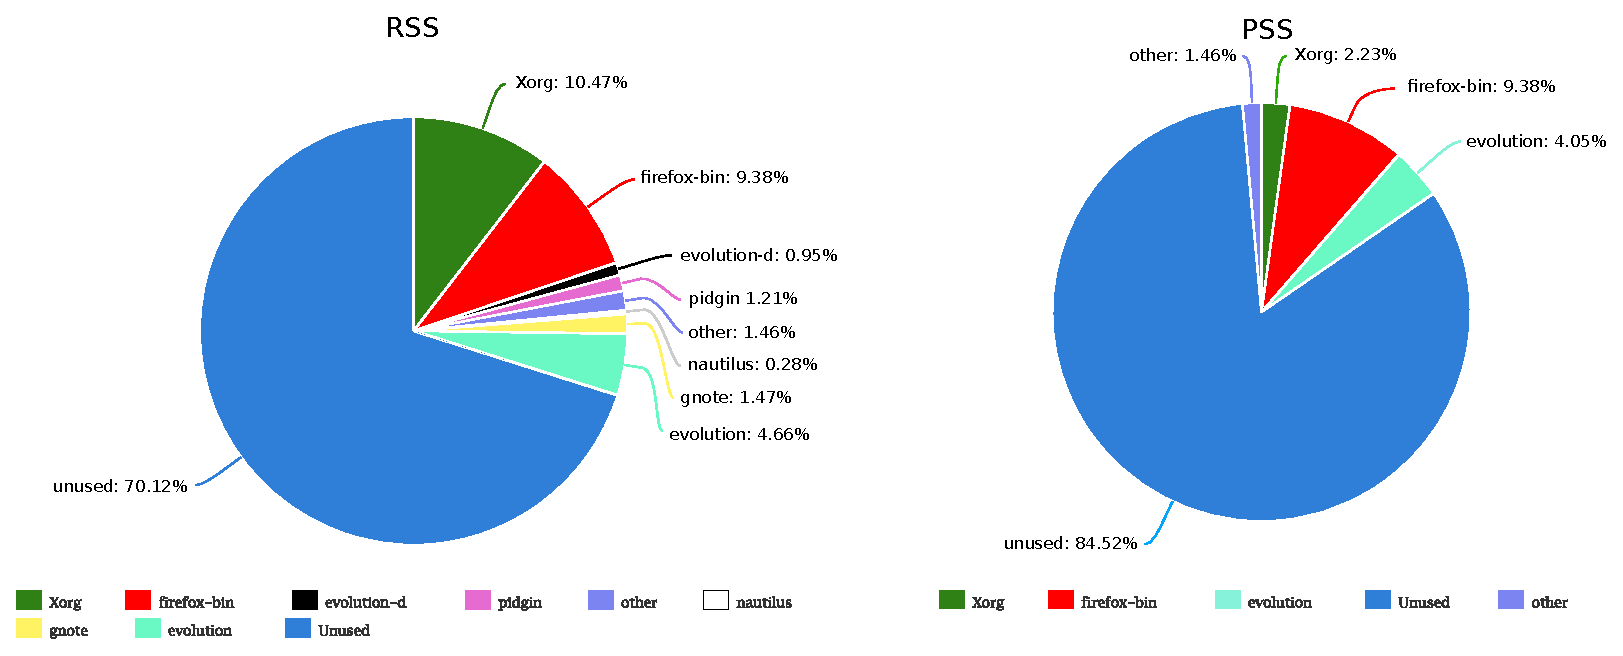
\includegraphics{obrazky-figures/smem.eps}}
		\caption{Rozdielny pohľad na vyťaženie RAM \cite{smem}}
		\label{smem_pss}
	\end{center}
\end{figure}

\subsection*{smartctl}
Užitočný nástroj monitorujúci zdravie fyzických diskov či už rotačných alebo nepohyblivých flash diskov. K~zisteniu stavu disku využíva monitorovací systém S.M.A.R.T., ktorý detekuje a~posiela správy o~rôznych ukazateľoch spoľahlivosti v~snahe predvídať zlyhania. Každá hodnota S.M.A.R.T. má svoj identifikátor, aktuálnu hodnotu a~najhoršiu \mbox{dosiahnutú hodnotu}. Umožňuje zistiť počet zapnutí diskov, problém so sektormi, problém s~radičom, teplotu disku a~iné. \cite{performance-monitor-book} 

\subsection*{ip}
Týmto nástrojom môžeme zistiť aktuálnu konfiguráciu sieťových rozhraní, taktiež umožňuje vykonávať zmeny na~rozhraniach, ako napríklad zmena IP adresy, brány \mbox{a~MAC adresy} \cite{text-utils-book}. Z~výpisu môžeme tiež vyčítať počet prijatých a~odoslaných paketov na~rozhraniach. Tento nástroj nahrádza zaužívaný program \texttt{ifconfig}.

\subsection*{blkid a lsblk}
Tieto dva programy umožňujú zobraziť informácie o~pripojených blokových zariadeniach, a to predovšetkým ich umiestnenie v~adresári \texttt{/dev}, ich univerzálny identifikátor UUID, label zariadenia, typ súborového systému, prípadne číslo partície \cite{text-utils-book}.

\subsection*{lsusb a lspci}
Program \texttt{lsusb} slúži k~zisteniu pripojených USB zariadení pričom o~nich poskytuje informácie ako identifikačné číslo výrobcu zariadenia, modelu a jeho názov. Na zistenie zariadení pripojených cez zbernicu PCI a jej novších derivátov slúži program \texttt{lspci}. \cite{text-utils-book}

\subsection*{df}
Pre jednoduché zistenie množstva zabraného priestoru na sekundárnych a terciárnych pamäťových zariadeniach môžeme použiť textovú utilitu \texttt{df} \cite{performance-monitor-book}.   

\section{Syslog}
V~dnešnom svete plnom počítačov, sieťových prvkov a~počítačových periférií vzniká veľké množstvo záznamov o~ich činnosti, ktoré majú informatívny, respektíve ladiaci charakter alebo oznamujú rôzne poruchy a~chyby pri~činnosti softvéru a~hardvéru. Tieto informácie je často nutné zaznamenávať nielen lokálne na~zariadeniach, ale aj posielať počítačovou sieťou na~centralizované miesto určené na~analýzu týchto informácií. Z~tohto dôvodu vznikol štandard syslog, ktorý zaznamenáva programové správy a~umožňuje ich posielať po~počítačovej sieti na~syslog server.

Protokol syslog je typu klient/server, pričom úlohu klienta zastáva zariadenie, ktoré generuje logovacie správy a~posiela ich na~server, na~ktorom beží syslog démon \cite{pro-admin-book}. Týmto syslog démonom alebo serverom môže byť aj zariadenie generujúce samotné syslog správy. Na~prenos po~počítačovej sieti využíva protokoly transportnej vrstvy TCP a~UDP, pričom je možné posielané dáta zabezpečiť pomocou SSL/TLS \cite{rfc-syslog}, keďže neraz obsahujú citlivé informácie.

Pre správne fungovanie rôznych implementácií syslog musíme mať na~všetkých zariadeniach správne nastavený čas \cite{pro-admin-book}. Na presné nastavenie času a~zároveň jeho pravidelnú synchronizáciu musíme na~počítačoch alebo sieťových prvkoch nastaviť NTP server. \mbox{Aktuálny čas} pomáha k~lepšiemu zisteniu poruchy a~umožňuje odhaliť sériu závislých chýb na~viacerých zariadeniach.

Súčasťou generovaných správ syslog je okrem času, kedy udalosť nastala taktiež zariadenie (Facility), úroveň (Severity level) a~dodatočné textové informácie. Každé zariadenie má unikátny kód a~kľúčové slovo, ktoré špecifikuje typ programu v~syslog správe. \mbox{Zároveň je}~pri~každej správe definovaná úroveň, respektíve priorita, ktorá udáva mieru závažnosti informácie. \cite{pro-admin-book} \cite{rfc-syslog}
\\\\
Typy priorít zostupne \cite{rfc-syslog}:
\begin{itemize}
	\item Emergency
	\item Alert
	\item Critical
	\item Error
	\item Warning
	\item Notice
	\item Info
	\item Debug\\
\end{itemize}
\noindent
Príklady zariadení \cite{pro-admin-book}:
\begin{itemize}
	\item auth\,--\,správy súvisiace s~bezpečnosťou
	\item authpriv\,--\,správy riadenia prístupu
	\item cron\,--\,správy generované cronom/plánovačom
	\item daemon\,--\,správy démonov a~procesov
	\item kern\,--\,správy jadra systému
	\item mail\,--\,správy súvisiace s~elektronickou poštou\\
\end{itemize}


%\chapter{Existujúce riešenia}
\section{Nagios}
Nagios je populárny open source program na sledovanie systému, počítačovej siete a~infraštruktúry \cite{nagios-web}. Primárne je vyvíjaný pre~operačné systémy Linux, Unix a~Unix\,--\,like. Od jeho vzniku v~roku 2002 si získal veľký trhový podiel medzi monitorovacím softvérom najmä vďaka jeho bezplatnosti, použitiu licencie GNU GPL, ale hlavne dobrej podpore a~množstvu oficiálnych a~neoficiálnych rozšírení.

Vďaka rozsiahlej dokumentácií a~dobrej podpore je inštalácia tohto monitorovacieho programu veľmi jednoduchá, no na~správne fungovanie je potrebná rozsiahla konfigurácia, ktorá zaberá množstvo času. Diagram činnosti systému Nagios môžeme vidieť na~obrázku č. \ref{nagios_scheme}.

Po nainštalovaní a~nakonfigurovaní je dostupné grafické užívateľské rozhranie cez~webový prehliadač \cite{nagios-web}. Toto užívateľské rozhranie je personalizovateľné a~zobrazuje rôzne dashbordy s~informáciami o~stave sieti, počte a~druhu upozornení, vyťaženie zdrojov staníc a~množstvo ďalších informácií.

Medzi nevýhody tohto softvéru patrí zastaralé používateľské rozhranie, neľahká konfigurácia a~nutnosť serveru s~veľkým množstvom pamäte.

\begin{figure}[H]
	\begin{center}
		\scalebox{0.6}{\includegraphics{obrazky-figures/nagios_scheme.png}}
		\caption[caption without footnote, for lof]{Princíp činnosti Nagios\footnotemark}
		\label{nagios_scheme}
	\end{center}
\end{figure}
\footnotetext{http://www.linux-magazin.de/news/nagios-plugins-in-version-2-0/}
\section{Zabbix}
Zabbix patrí k~populárnym real-time nástrojom na~monitorovanie počítačovej siete a~ap\-li\-ká\-cií \cite{zabbix-doc}. Tak ako nástroj Nagios je viac zameraný na~monitorovanie počítačovej siete, no zvláda taktiež sledovanie serverov a~služieb na~nich bežiacich. Veľkou devízou Zabbixu oproti Nagios bola možná konfigurácia pomocou grafického rozhrania, čo však už dnes neplatí, pretože ju už oba nástroje podporujú.

Na ukladanie dát používa Zabbix relačné databáze, ako napríklad MySQL, PostgreSQL alebo Oracle SQL, je napísaný v~programovacom jazyku C a~na jeho frontend je využitý jazyk PHP \cite{zabbix-doc}.

Zabbix je možné používať ako na~GNU/Linux, tak aj na~systémoch Windows. Umožňuje sledovať služby ako SMTP, HTTP a~iné, vyťaženie CPU, diskov a~siete. Naproti systému Nagios ponúka modernejšie a~intuitívnejšie grafické rozhranie a~jednoduchšiu konfiguráciu. 
\chapter{Návrh}
\label{navrh}
\section{Požiadavky na aplikáciu}
Kľúčovými vlastnosťami výsledného programu na~monitorovanie uzlov v~clusteri sú nenáročnosť z~pohľadu výkonu a~množstva prenesených dát po~sieti, možnosť spustenia na~rôznych GNU/Linux distribúciách, modulárnosť, jednoduchosť vytvorenia nových skriptov a~integrácia už existujúcich skriptov.

Prenositeľnosť naprieč rôznymi distribúciami GNU/Linux je taktiež dôležitou požiadavkou, preto bol na~implementáciu vybraný jazyk \mbox{Python}, ktorý okrem bezproblémovému chodu na~všetkých distribúciách je dobre editovateľný a~čitateľný pre~budúcich používateľov, ktorí si budú môcť pridávať vlastné skripty a~meniť správanie aplikácie.

\noindent
\\
Samotný monitorovací nástroj bude rozdelený do piatich častí, a to:
\begin{itemize}
	\item Inštalačný skript\,--\,\texttt{install.py}
	\item Riadiaci monitorovací a notifikačný skript\,--\,\texttt{linmon.py}
	\item Monitorovacie moduly v~zložke \texttt{monitoring\_scripts}
	\item Moduly monitorujúce rsyslog záznamy v~zložke \texttt{syslog\_scripts}
	\item Pomocné skripty v~zložke \texttt{aux\_scripts} 
\end{itemize}

Monitorovací program je hierarchicky rozdelený z~dôvodu ľahšej implementácie nových skriptov a~tiež kvôli využitiu skriptov ako samostatné programy. Zoznam skriptov a~ich zverených úloh sú popísané v~prílohe \ref{skripty}. 

\begin{figure}[H]
	\begin{center}
		\scalebox{0.6}{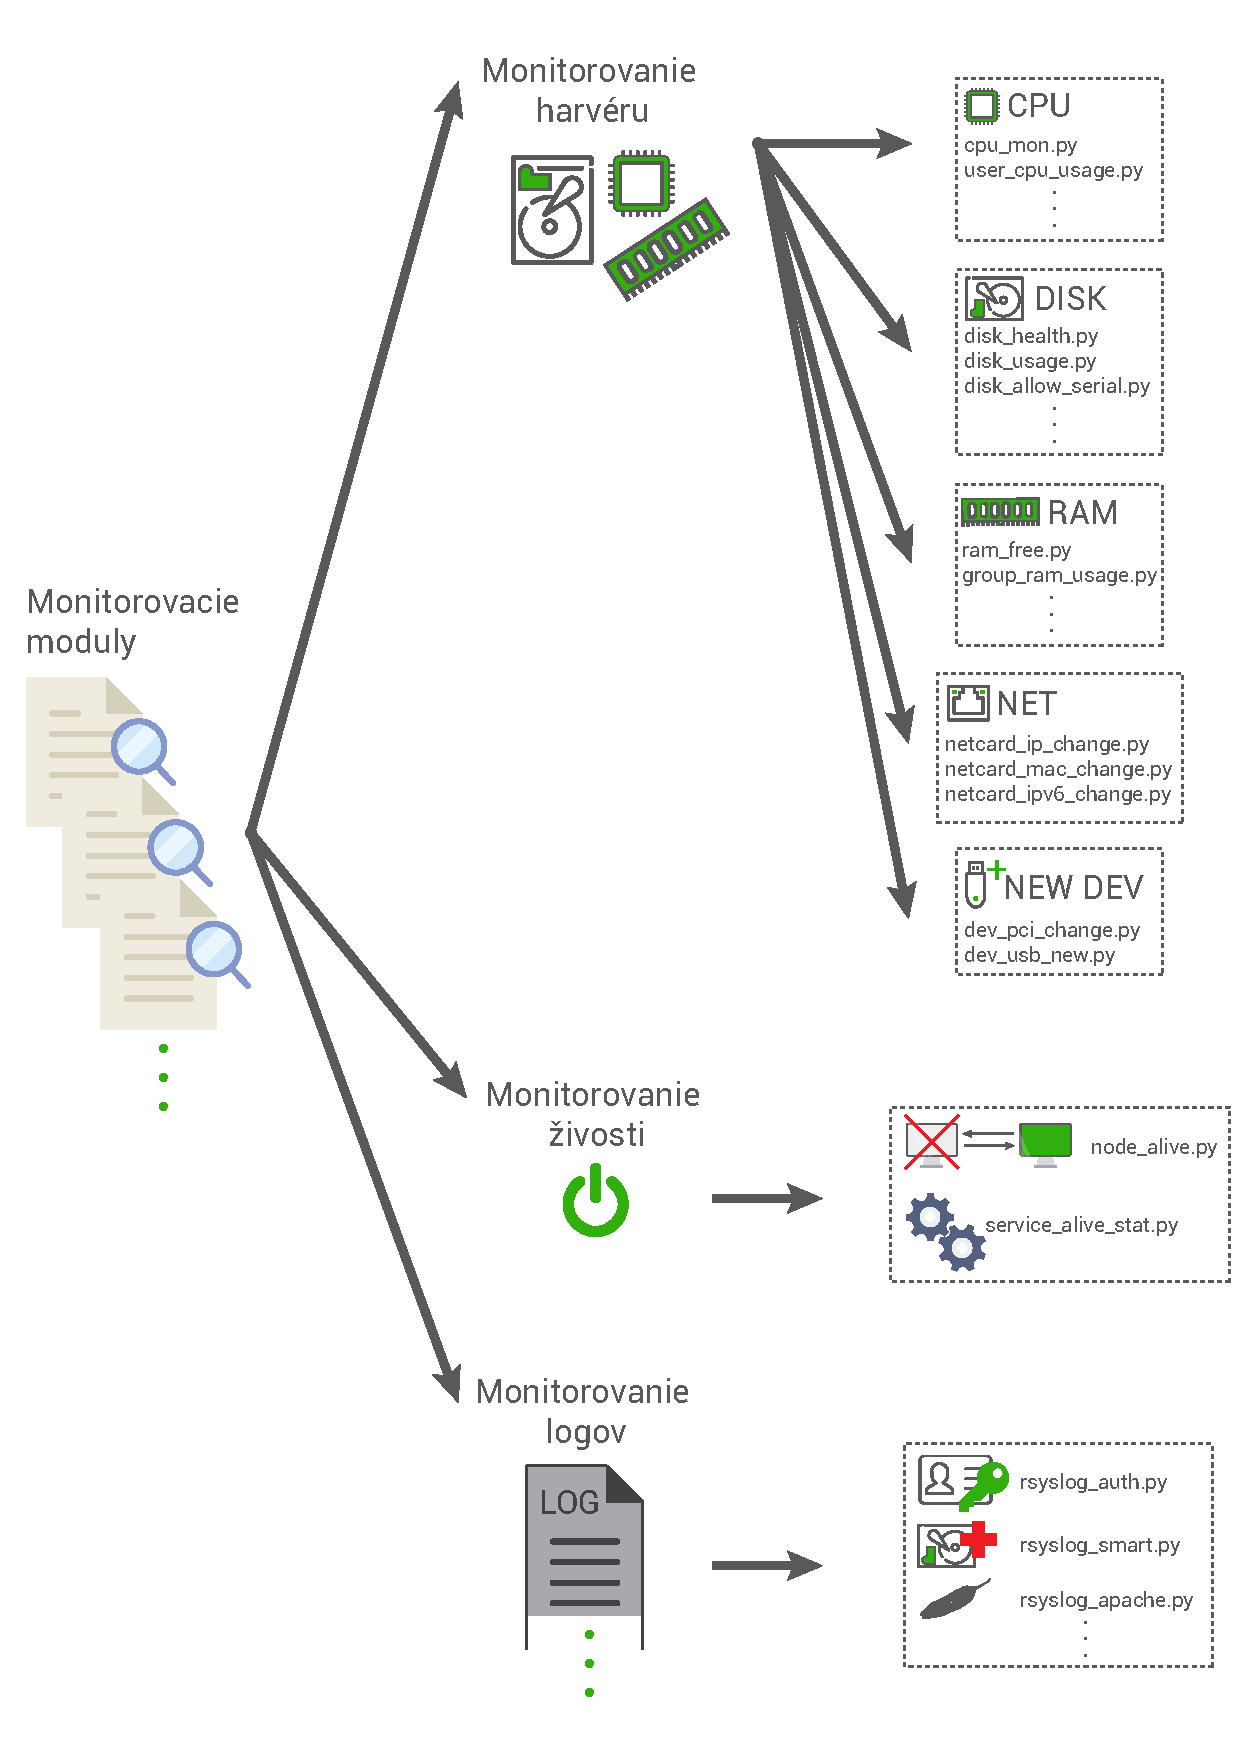
\includegraphics{obrazky-figures/script_classes.pdf}}
		\vspace{-2em}
		\caption{Hierarchické rozdelenie monitorovacích modulov}
		\label{script_classes}
	\end{center}
\end{figure}

Pre bezproblémovú integráciu nových skriptov do~monitorovacieho nástroja bude vypracovaná šablóna s~manuálom, ako vytvárať skripty pre~bezproblémovú funkcionalitu v~monitorovacom programe a~to najmä definícia výstupov nutná pre~prácu hlavného skriptu.

Ako môžeme vidieť v~prílohe \ref{skripty}, administrátor systému je vždy oboznámený so zmenou stavu alebo chybou, ktorá nastala. Na tento účel bude použitá notifikácia pomocou \mbox{emailu}, kde bude okrem informácie, že skript zlyhal aj detailný výstup.

\section{Odlišnosti oproti existujúcim riešeniam}
Monitorovací softvér ako Nagios a Zabbix opísaný v~kapitole \ref{monitorovanie} majú nesporné výhody v~podpore a širokej nasadenosti. No pre niektoré vlastnosti je na monitorovanie zariadení nevhodný, ťažkopádny a zbytočne komplexný. V~prvom rade monitorovací nástroj Linmon nepotrebuje databázy na uchovania monitorovacích informácií. 

Častokrát výrobca alebo predajca zariadenia, ktoré potrebujú administrátori monitorovať dodáva svoje proprietárne monitorovacie riešenia a neumožňuje inštaláciu iných monitorovacích programov alebo umožňuje za cenu straty záruky. Pri týchto obmedzeniach však často umožňuje spúšťanie Python skriptov. Z~tohto dôvodu je nástroj Linmon vhodnejším kandidátom na monitorovanie ako Nagios a Zabbix. 

Zároveň umožňuje jednotné rozhranie pre monitorovacie skripty a zoskupenie notifikačných správ pri nájdení abnormálnych hodnôt, čo neumožňujú separátne úlohy v~plánovači \texttt{cron}. Súčasťou takmer každej distribúcie GNU/Linux je interpret jazyku Python a  program na prenos správ elektronickej pošty \texttt{sendmail}, ktoré sú zároveň jedinými nutnými prerekvizitami na chod nástroja.

V~neposlednom rade veľkou výhodou je aj minimalistickosť a nenáročnosť na strane príjemcu notifikačných správ. Nagios a Zabbix potrebujú pre zobrazenie informácií webserver, no nástroju Linmon postačuje email klient na akomkoľvek zariadení alebo dokonca iba unix terminál, na ktorom je taktiež možné správy zobraziť. 

\section{Inštalácia}
Inštalačný skript je zodpovedný za zavedenie monitorovacieho nástroja do systému, čo zahŕňa uloženie konfiguračných dát pre zariadenie, nakopírovanie monitorovacích modulov a ich konfiguračných súborov do systému a taktiež je ním možné monitorovací nástroj odinštalovať. Prácu tohto skriptu ilustruje vývojový diagram \ref{script_install}.

Podľa konvencií hierarchie súborového systému má byť pre vlastné binárne súbory a skripty použitý priečinok \texttt{/opt} a pre ich konfiguračné súbory zasa \texttt{/etc/opt} \cite{file-hierarchy}. Preto bude ako predvolená inštalačná zložka nástroja Linmon \texttt{/opt/linmon/} a ich konfiguračné súbory budú pri inštalácií zavedené do \texttt{/etc/opt/linmon/}.  

Z~dôvodu uchovania nastavení zadaných v~príkazovom riadku pri inštalácií je vytvorený konfiguračný súbor uzlu obsahujúci zoznam emailových adries určených na notifikáciu, cestu k~zložke so skriptami a ku konfiguračným súborom a cestu k~binárnemu súboru \texttt{sendmail}.

Na záver inštalácie je zaslaný informačný email, v~ktorom je hlavička, ktorá jednoznačne identifikuje zariadenie, na ktorom inštalácia prebehla a taktiež informácia o~úspešnosti inštalácie s~prípadnými chybami.

\begin{figure}[H]
	\begin{center}
		\scalebox{0.4}{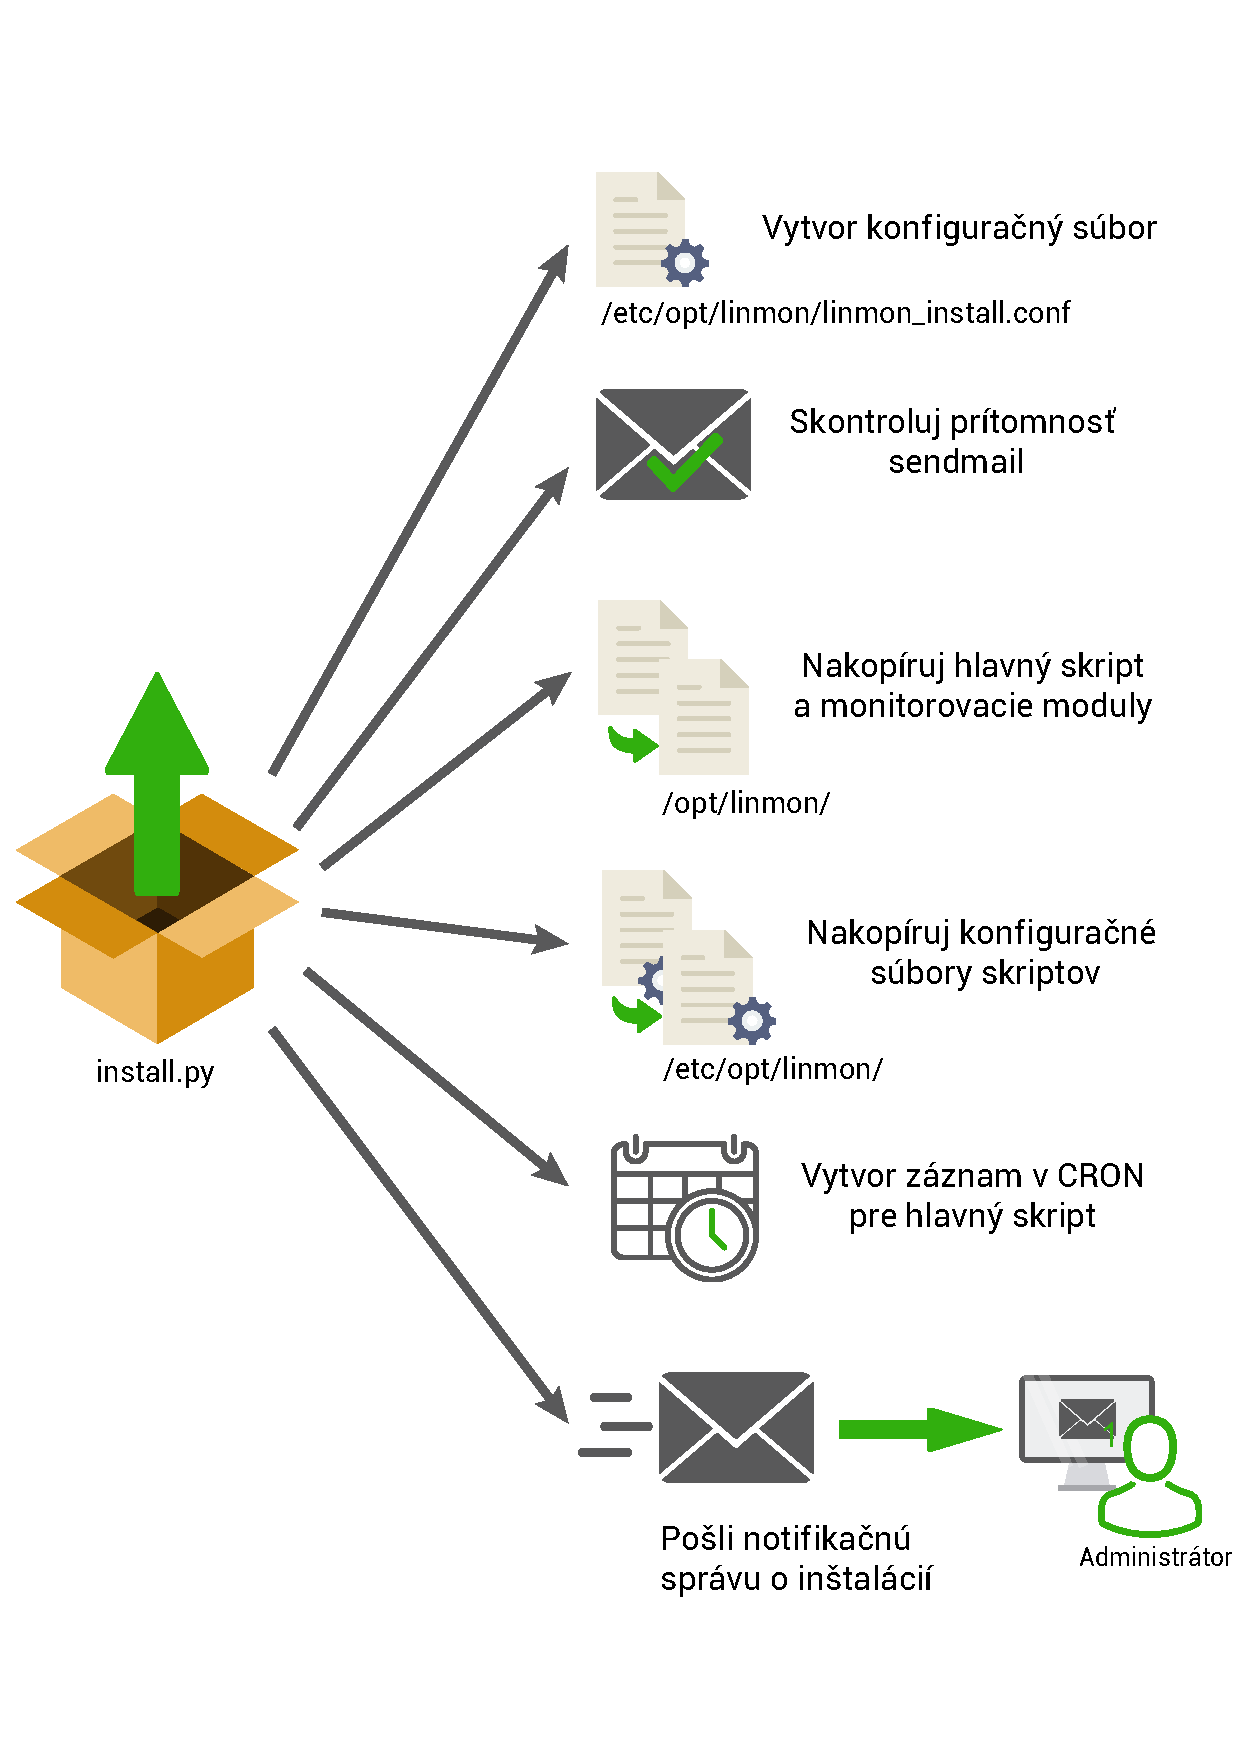
\includegraphics{obrazky-figures/install_pic.pdf}}
		\vspace{-2.5em}
		\caption{Zjednodušený pohľad na inštaláciu skriptu}
		\label{script_install_pic}
	\end{center}
\end{figure}
\begin{figure}[H]
	\begin{center}
		\scalebox{0.3}{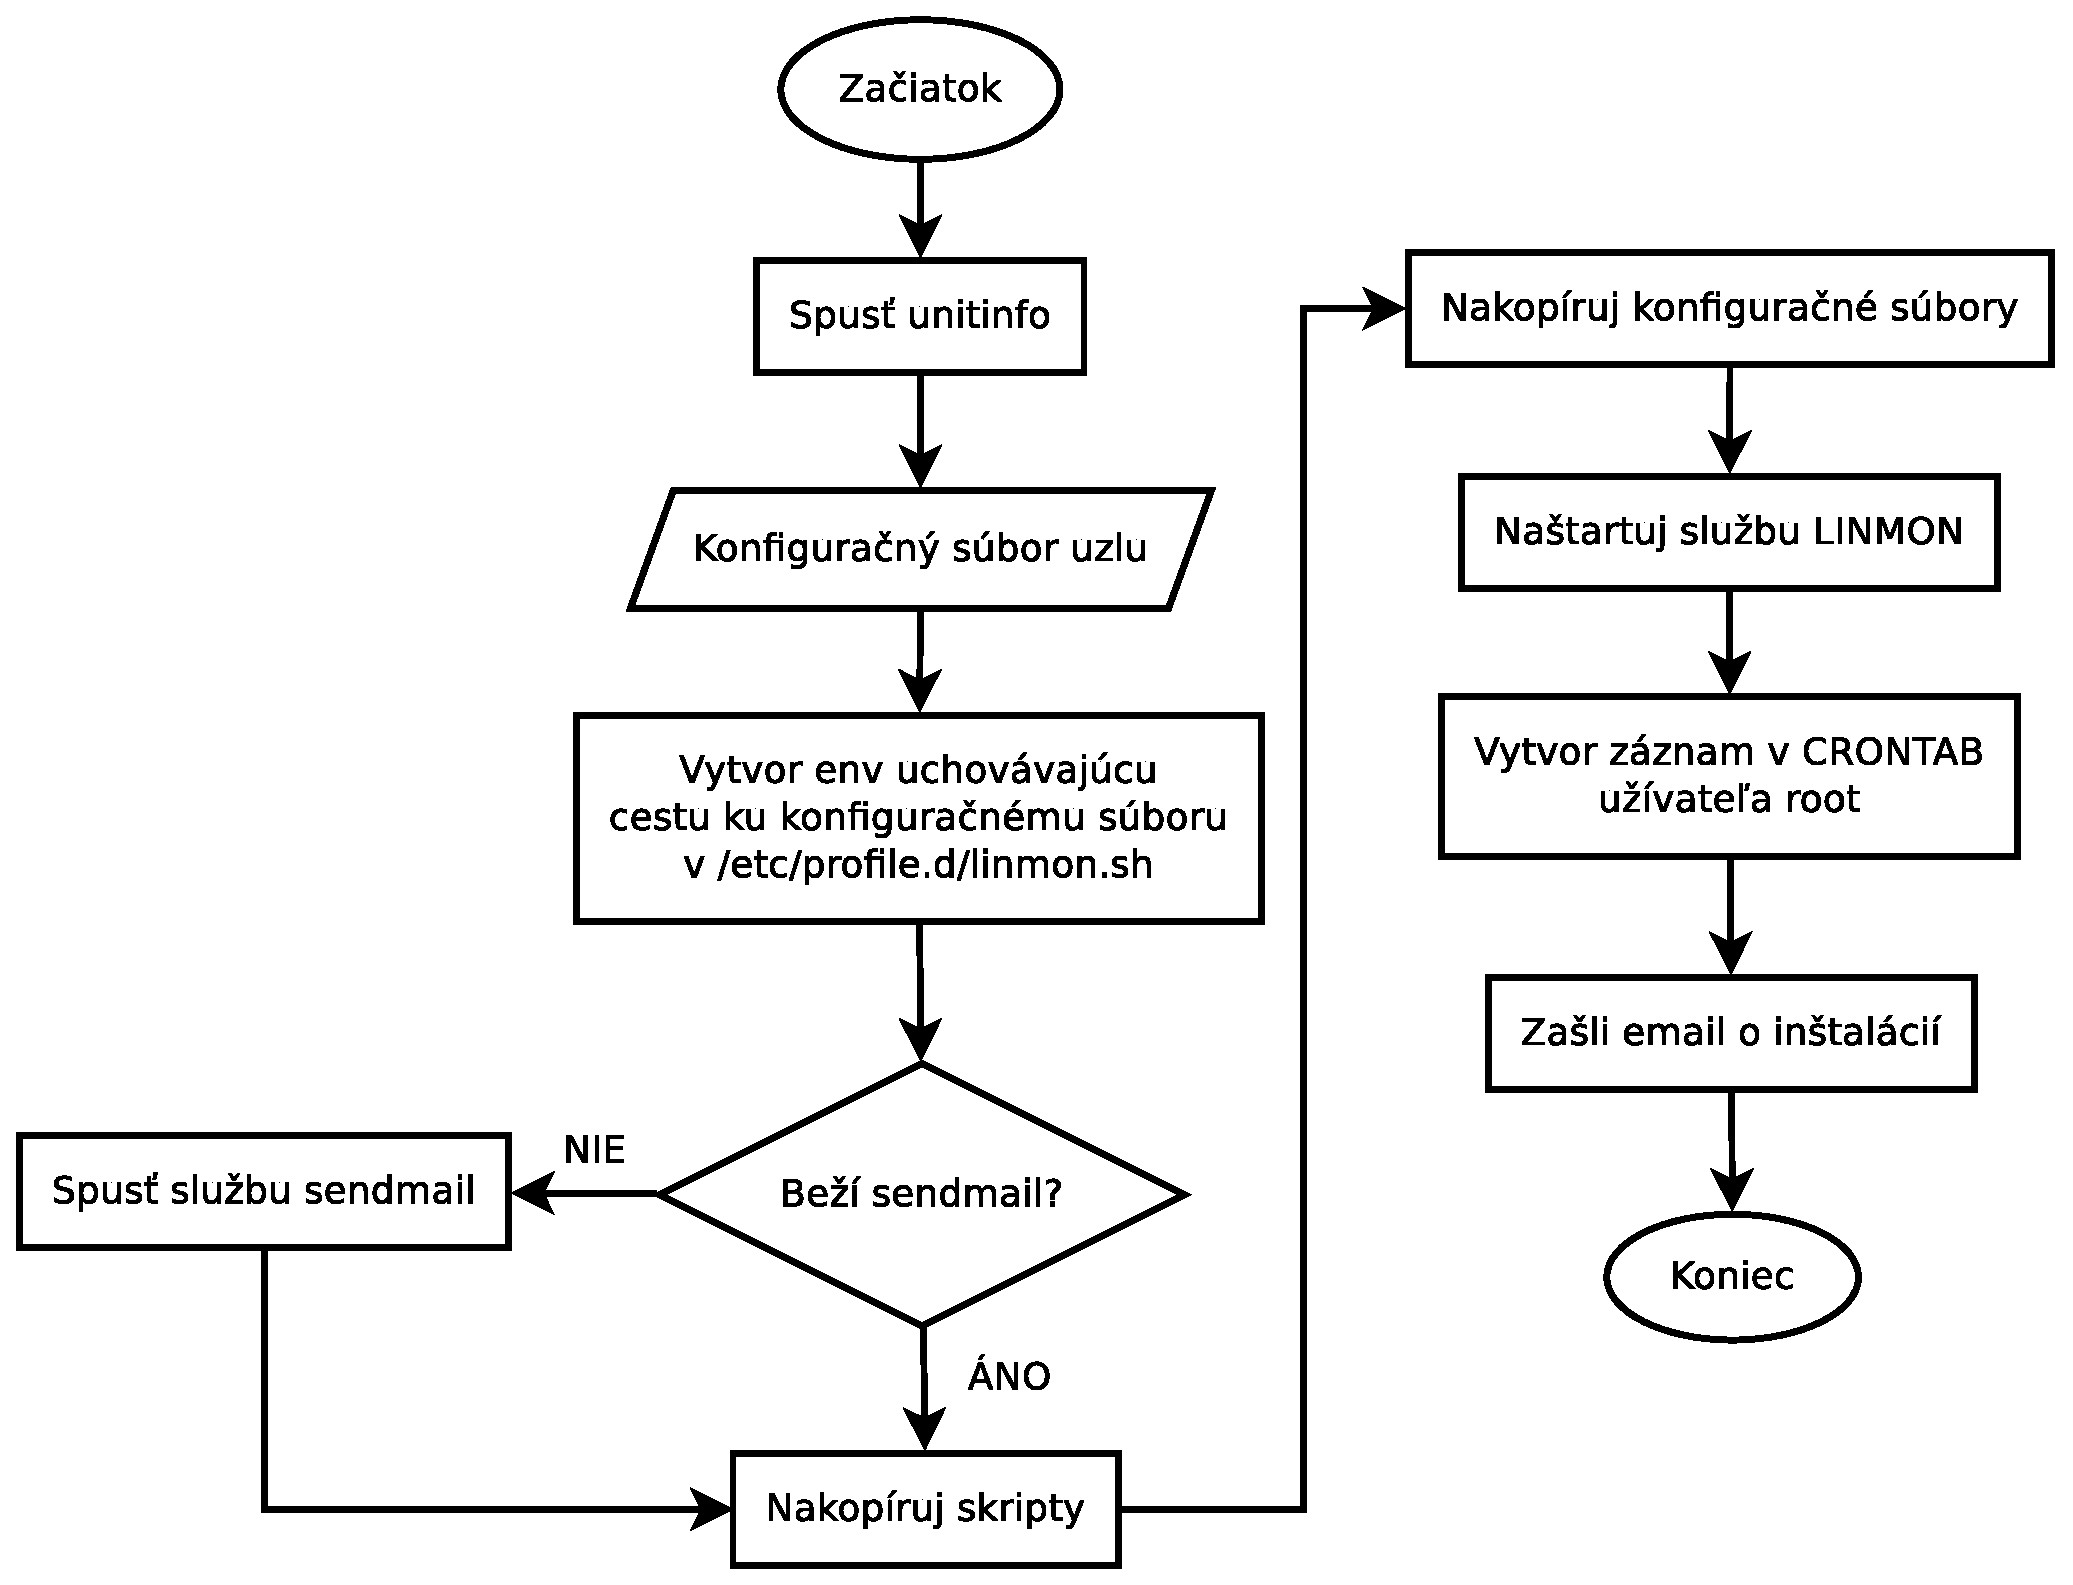
\includegraphics{obrazky-figures/install.eps}}
		\caption{Diagram počiatočnej inštalácie a~konfigurácie skriptu}
		\label{script_install}
	\end{center}
\end{figure}

\section{Hlavný skript}
\label{hlavny_skript}
Hlavný skript \texttt{linmon.py} sa stará o~spúšťanie definovaných skriptov (monitorovacích modulov) a následnú notifikáciu administrátora pri nájdení abnormálnych hodnôt monitorovacími modulmi.

Dôležitým faktorom pri~monitorovaní počítačov je zaistenie stáleho behu monitorovacieho skriptu. Táto požiadavka bude zaistená vložením skriptu do~plánovača \texttt{cron}, kde sa každých 5 minút overí chod skriptu a taktiež za pomoci init systému. Keďže sa každých 5 minút spustí program, treba zaistiť, že pokiaľ je už program spustený, tak nespustí monitorovacie moduly, pretože by mohlo prísť k~opakovanej notifikácií. Takéto správanie sa docieli umiestnením zámku na súbor \texttt{/var/run/linmon}.

Jednotlivé skripty popísané v~prílohe \ref{skripty} budú spúšťané z~hlavného skriptu v~pravidelných intervaloch, kde každý skript môže mať tento interval odlišný.

Po počiatočnom načítaní a naplánovaní spustenia monitorovacích modulov sa skript dostane do nekonečného cyklu, kde sa na základe času spúšťajú definované skripty, naplánujú sa ich ďalšie spustenia a v~prípade nájdenia abnormálnych hodnôt príde k~notifikácií administrátora.

\begin{figure}[H]
	\begin{center}
		\scalebox{0.55}{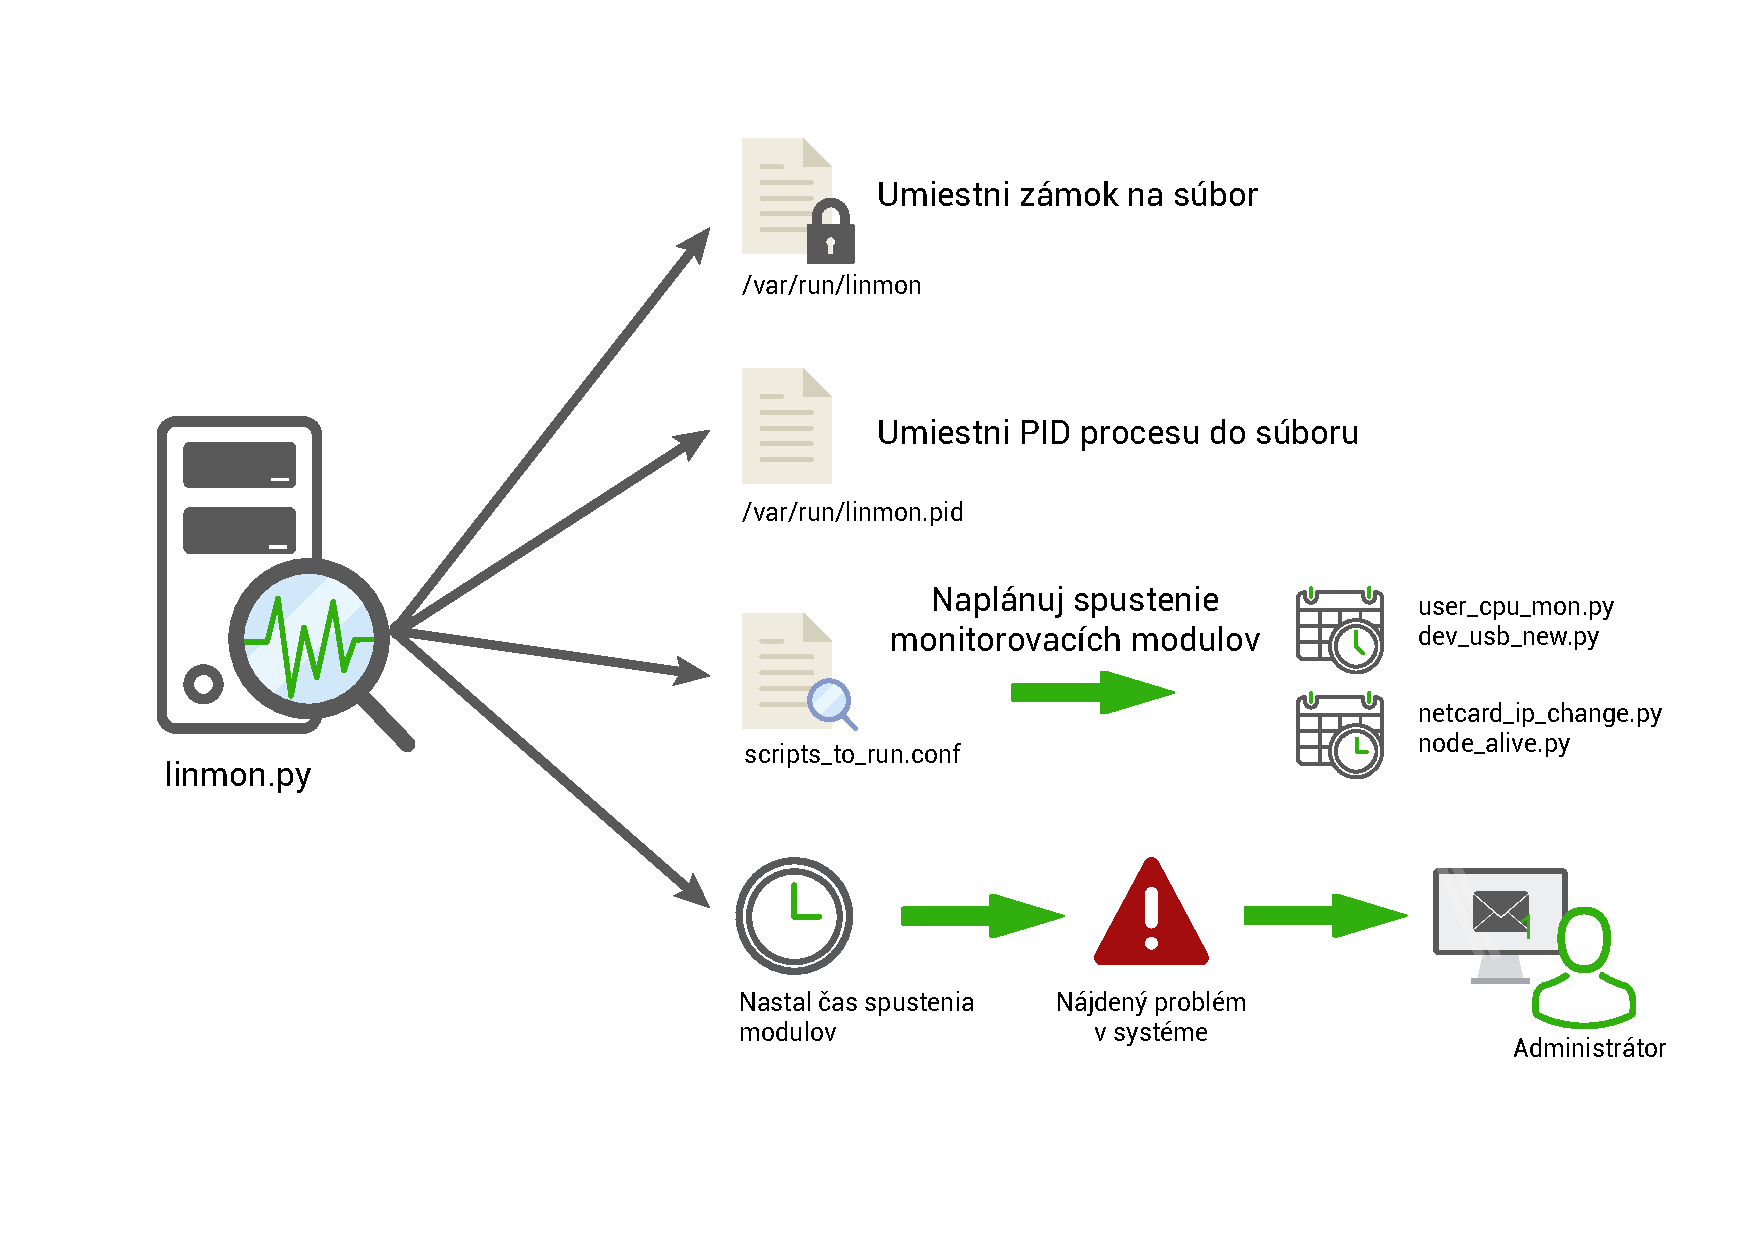
\includegraphics{obrazky-figures/linmon_pic.pdf}}
		\vspace{-5em}
		\caption{Zjednodušený pohľad na fungovanie hlavného skriptu}
		\label{linmon_main_pic}
	\end{center}
\end{figure}

\begin{figure}[H]
	\begin{center}
		\scalebox{0.35}{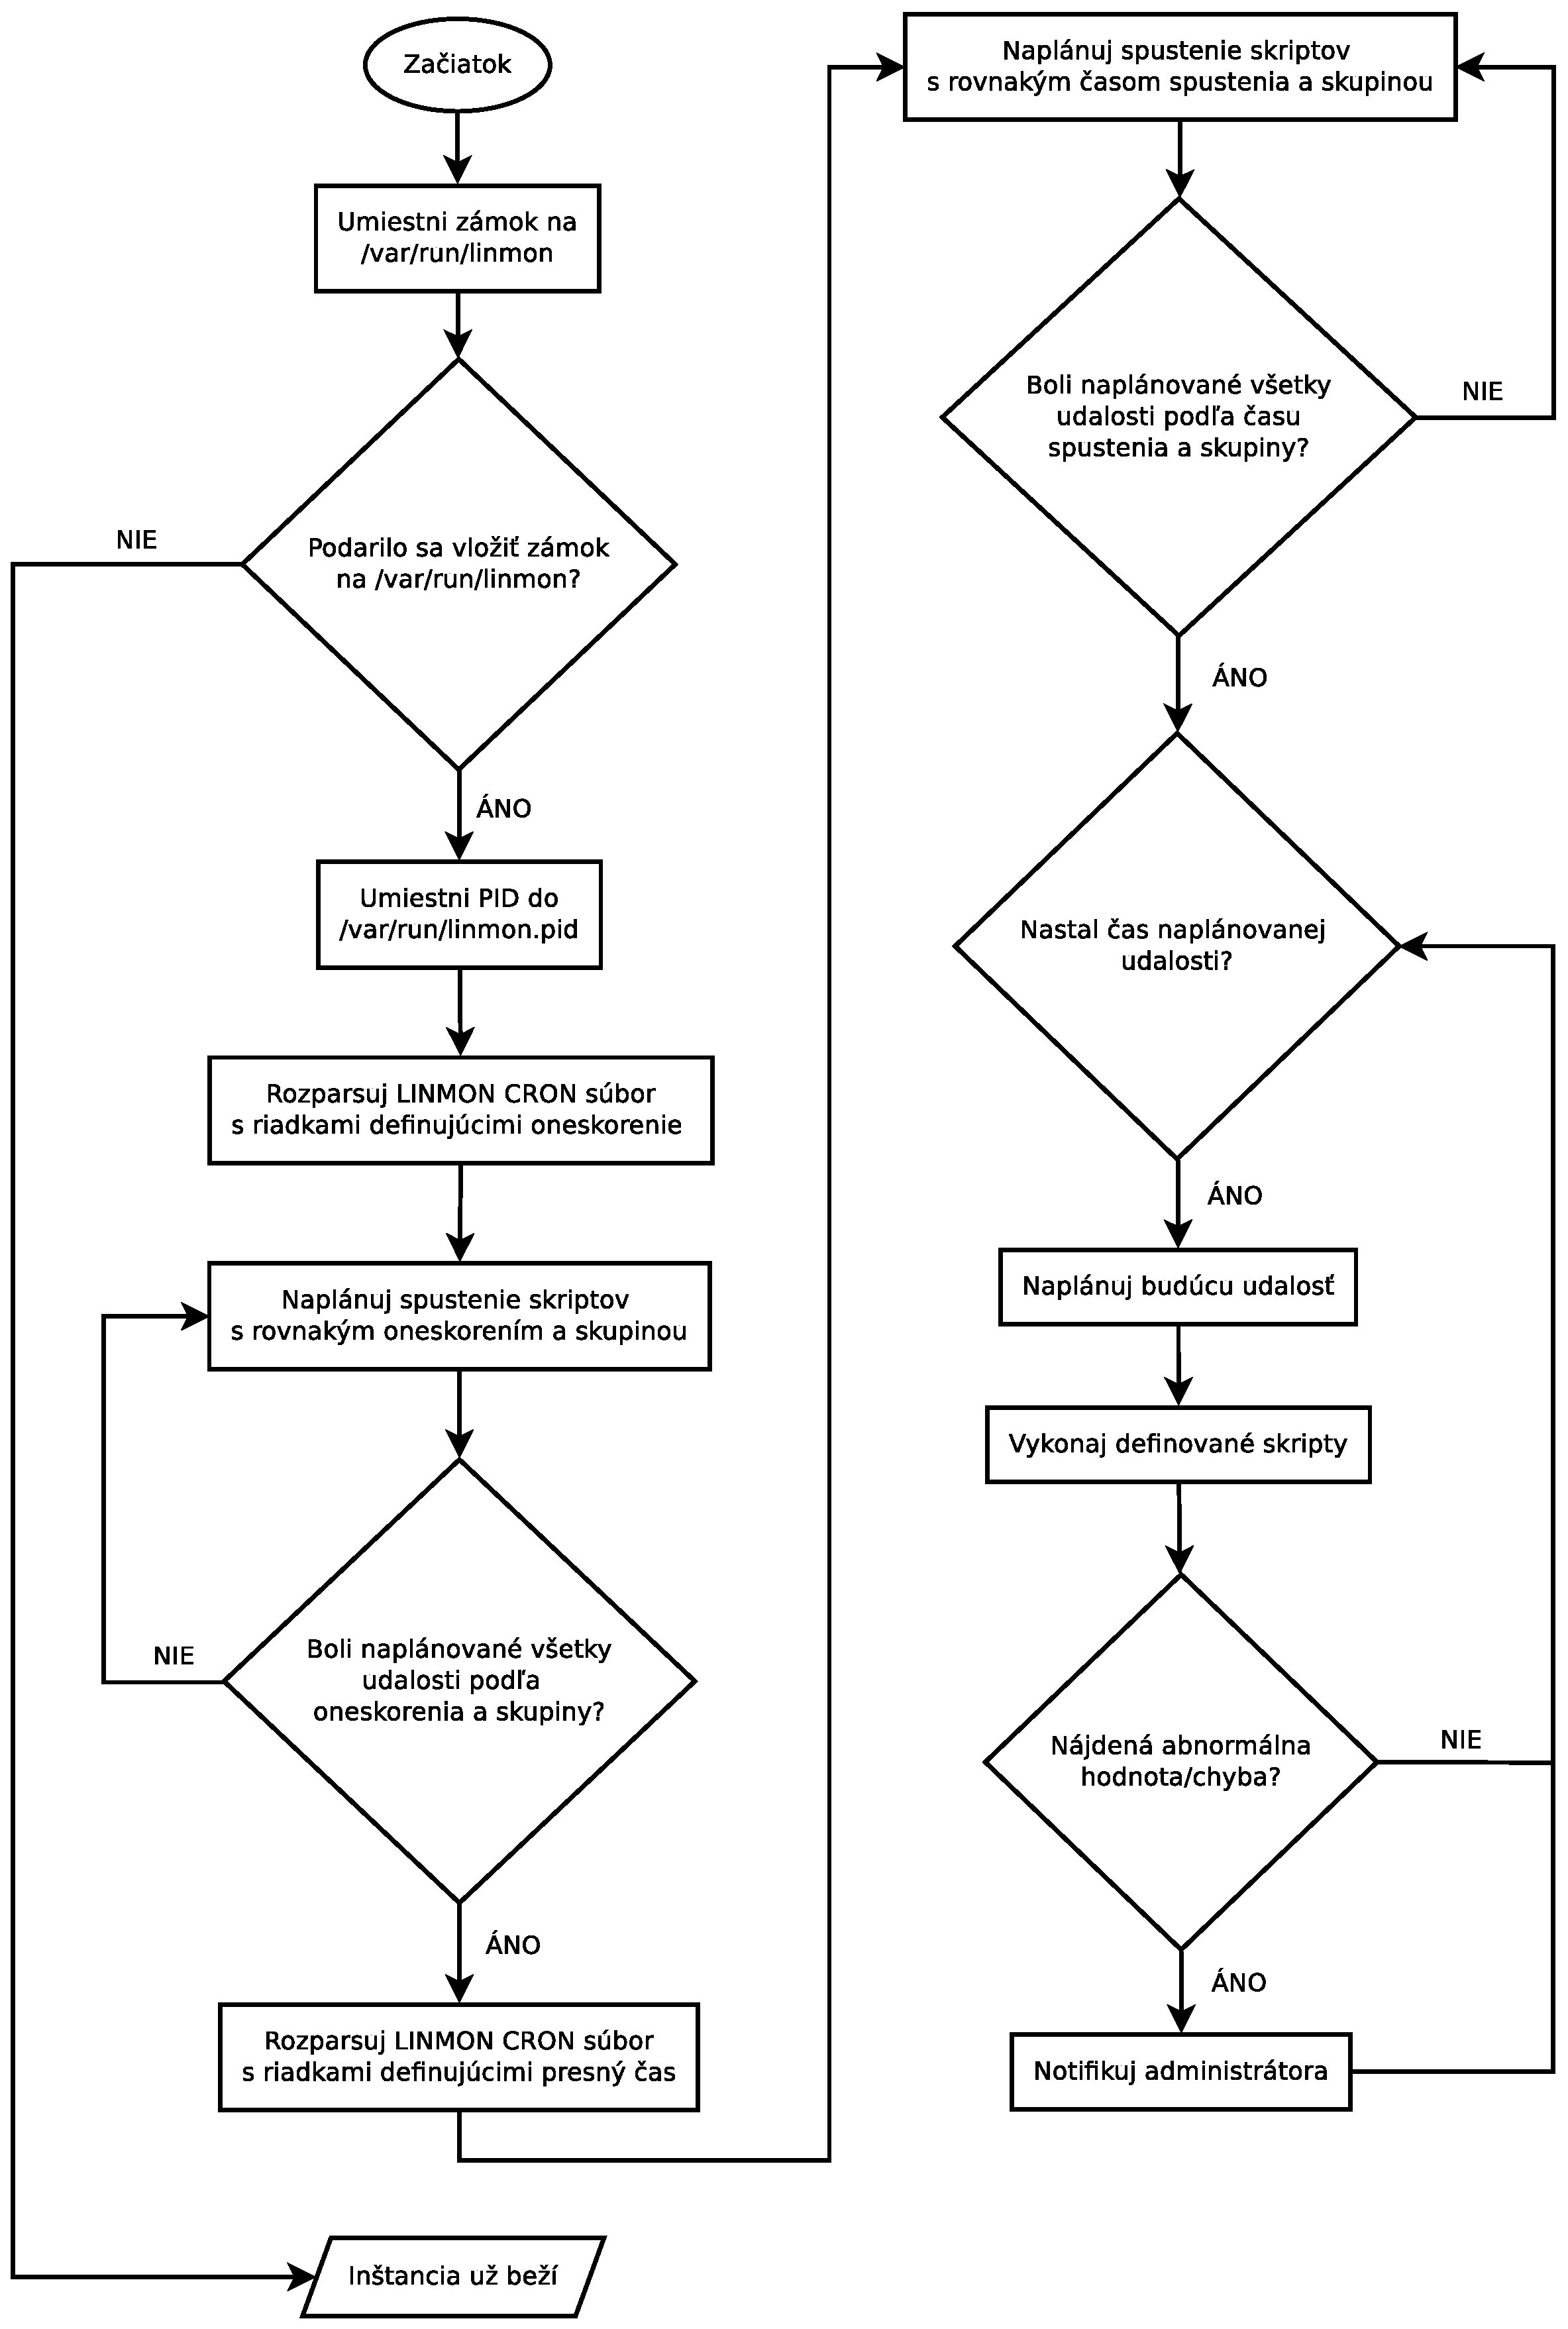
\includegraphics{obrazky-figures/linmon.eps}}
		\caption{Vývojový diagram hlavného skriptu}
		\label{linmon_main}
	\end{center}
\end{figure}

\subsection*{Maintenance mód}
Monitorovací skript bude spustený ako démon, teda bude bežať na pozadí a v~pravidelných intervaloch spúšťať monitorovacie moduly. No, ak počas monitorovania systému dôjde k~servisnému zásahu administrátora na~monitorovanom zariadení, môže to vyvolať reťaz notifikácií a~zahltenie poštovej schránky prijímajúcej notifikácie. Z~tohto dôvodu bude v~hlavnom skripte implementovaný tzv. maintenance mód, ktorým sa dočasne vypne monitorovanie a~zasielanie správ o~chybách. Vývojový diagram \ref{maintenance_mode} prezentuje činnosť tejto funkcie, pričom ako môžeme vidieť, je možné tento mód zapnúť a následne vypnúť po ukončení údržby alebo špecifikovať dobu, po ktorú bude bežať.
\\
\\
\begin{figure}[H]
	\begin{center}
		\scalebox{0.3}{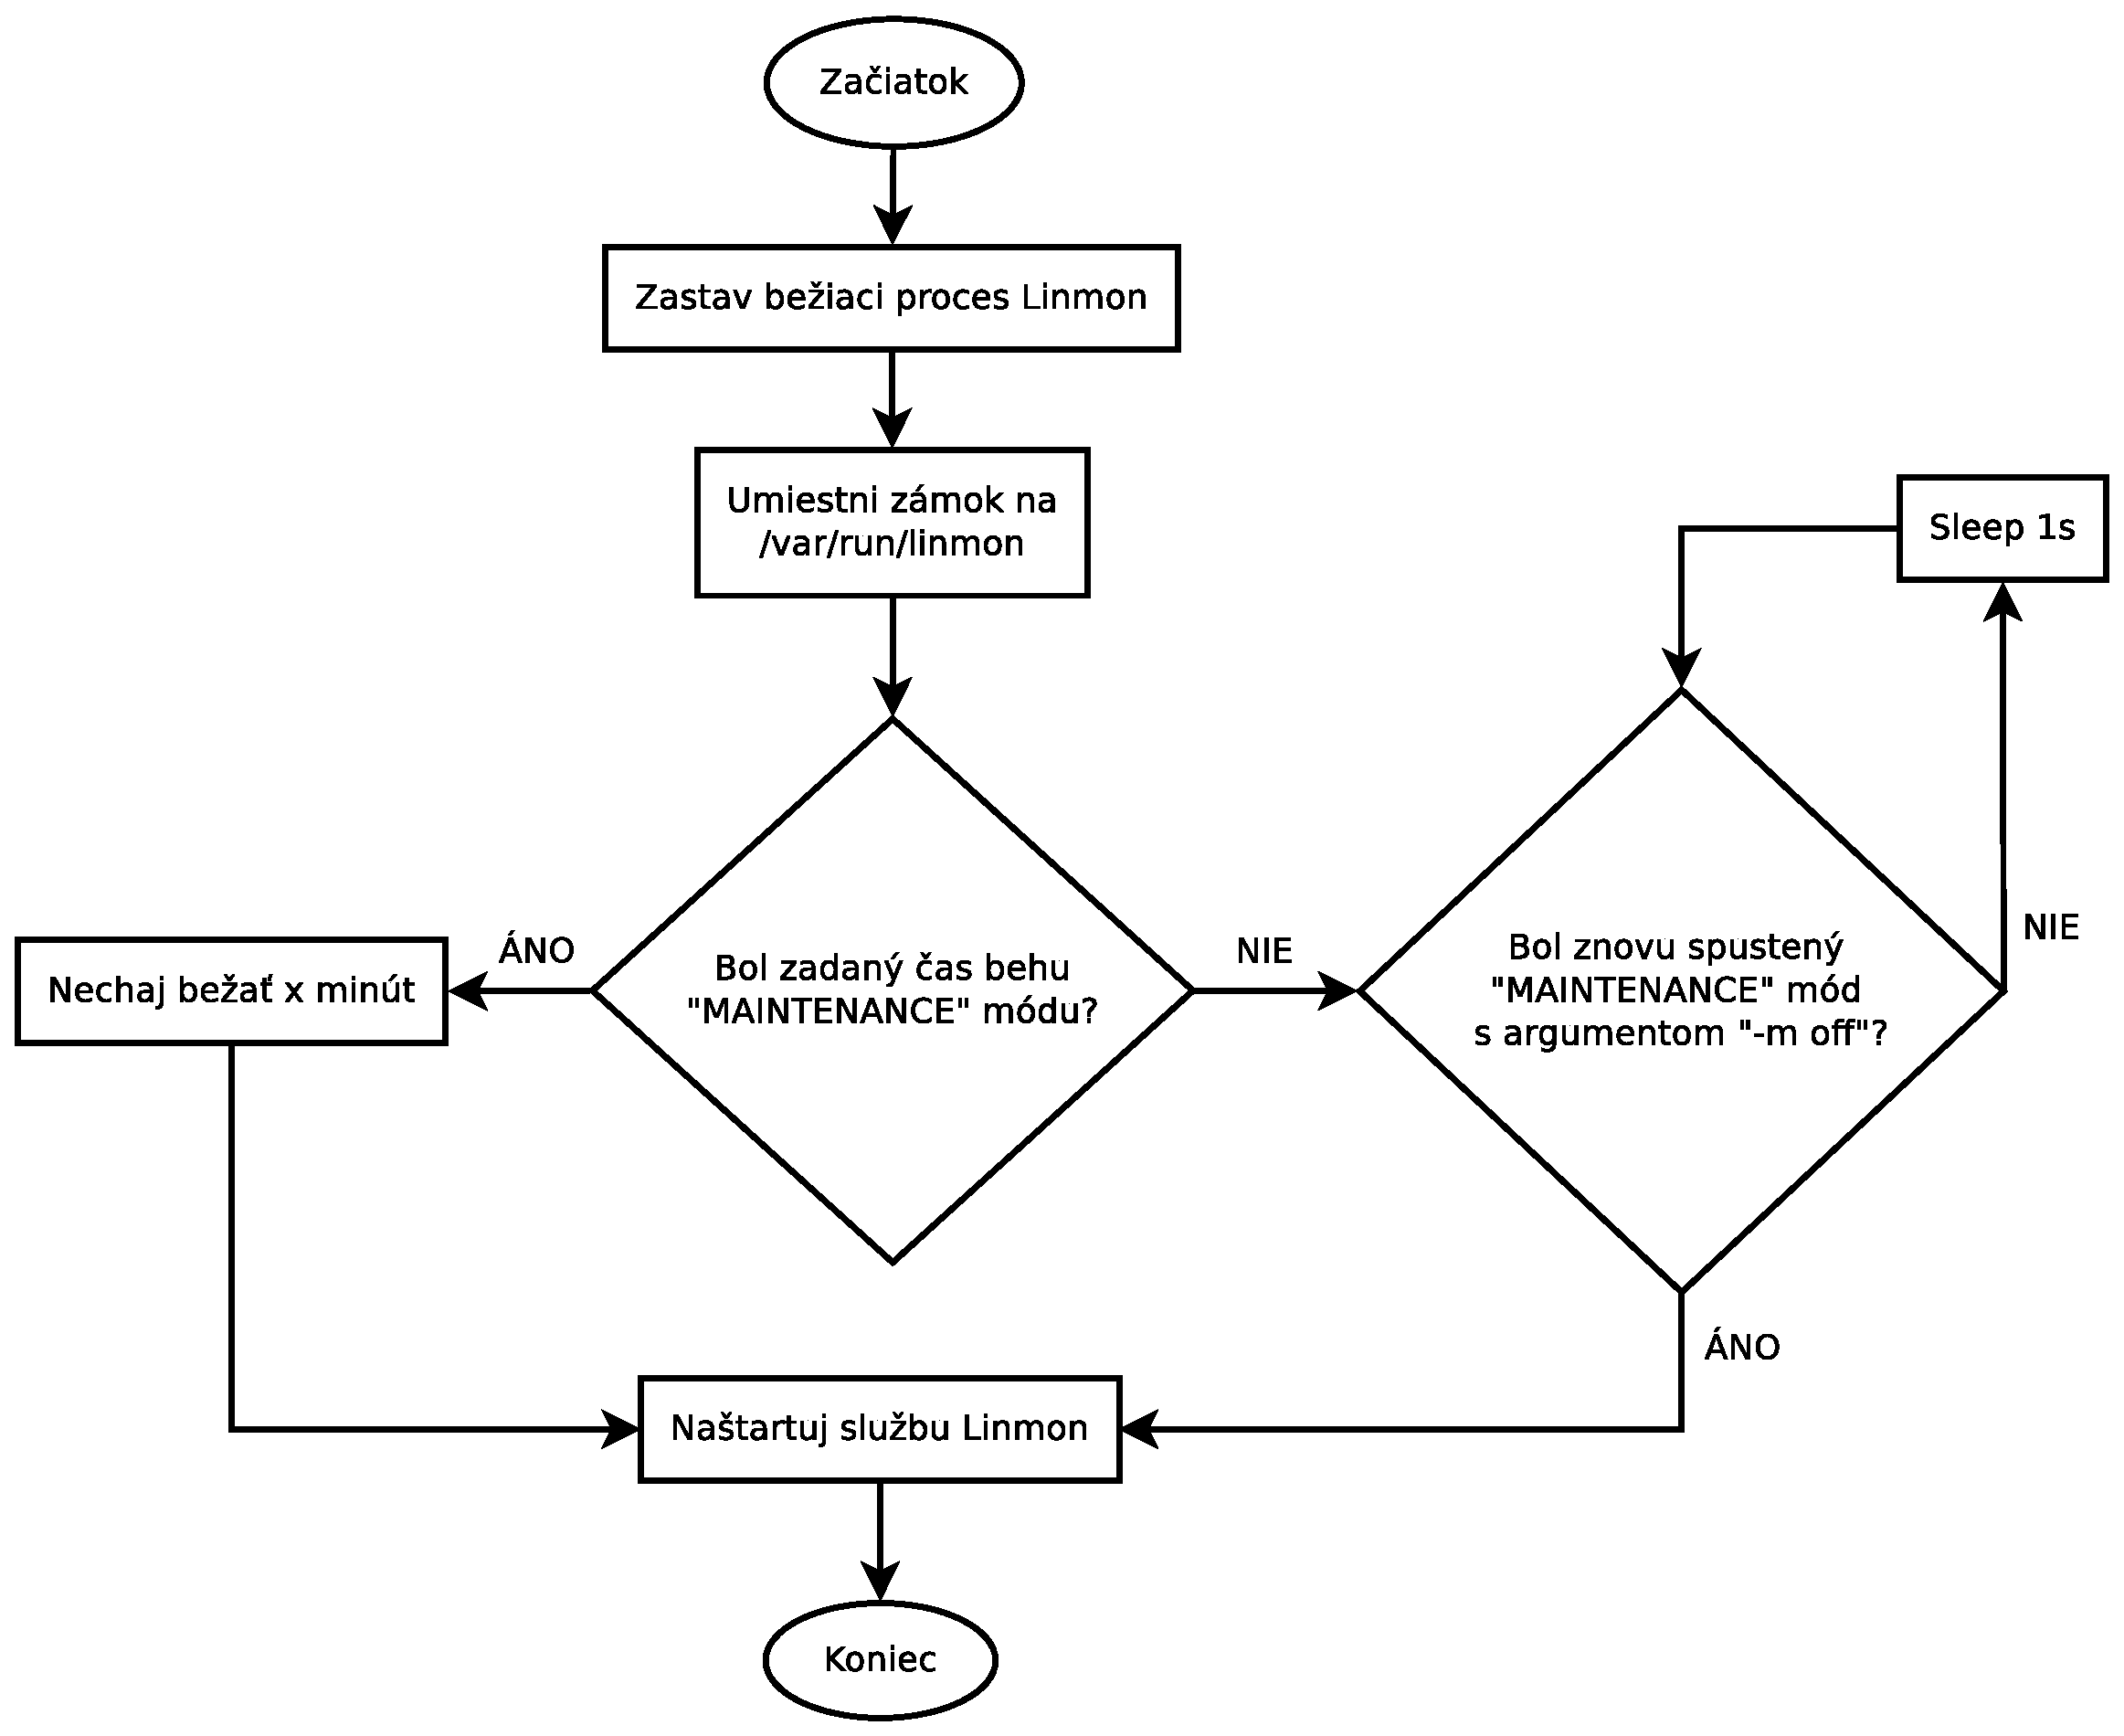
\includegraphics{obrazky-figures/maintenance.eps}}
		\caption{Vývojový diagram módu údržby}
		\label{maintenance_mode}
	\end{center}
\end{figure}

\chapter{Implementácia}
\label{implementacia}
V~tejto kapitole sa bližšie pozrieme na zaujímave pasáže a kľúčové prvky implementácie monitorovacieho a notifikačného programu \texttt{linmon.py},
taktiež si rozoberieme implementáciu monitorovacích modulov starajúcich sa o~sledovanie jednotlivých služieb alebo zdrojov výpočtového zariadenia. 

Ako implementačný jazyk pre túto bakalársku prácu bol vybraný skriptovací jazyk Python, ktorý je zväčša dostupný v~každej distribúcií GNU/Linux alebo je ho možné veľmi jednoducho doinštalovať. Na zaistenie čo najmenšieho zásahu do operačného systému, teda inštalácie a z~dôvodu zabránenia nekompatibility a konca vývoja rôznych knižníc boli v~implementácií použité iba vstavané knižnice jazyka Python dostupné od verzie 3.5.

\section{Hlavný skript Linmon}

Hlavný skript Linmon riadi jednotlivé monitorovacie moduly monitorujúce či už záznamy rsyslog alebo služby a zdroje. Je kompatibilný so súčasnými init systémami ako sú SystemD, SysV, Upstart. Nepretržitý chod skriptu je zabezpečený dvoma na sebe nezávislými spôsobmi popísanými v~podkapitole Zaistenie vysokej dostupnosti.  

\subsubsection*{Implementácia vlastného plánovača}
Ako už bolo spomenuté, skript Linmon iba spúšťa jednotlivé definované monitorovacie moduly, ktoré sa zameriavajú na jednu špecifickú oblasť monitorovania. Tieto moduly musia byť niekde vopred špecifikované, aby mal skript povedomie o~jednotlivých exekúciách.

\noindent
V~prvej fáze vývoja, respektíve návrhu aplikácie sa počítalo s~využitím vstavaného \mbox{linuxového} plánovača \texttt{cron}, od tohto smerovania bolo však upustené z~viacerých dôvodov, a to: 

\begin{itemize}
	\item  Skripty s~rovnakým naplánovaným časom spustenia by nemali údaje na výstupe v~rovnakom čase a nebolo by možné agregovať skripty naplánované v~rovnakom čase do jedného notifikačného emailu.
	
	\item Nemožnosť vytvorenia zoskupenia skriptov vrámci rovnakého času spustenia, teda pokiaľ by sme chceli v~rámci skriptov spustených každých 5 minút nedostať jednu agregovanú správu, ale rozdeliť v~rámci týchto piatich minút správy na dve alebo viac na základe nejakej značky.
	
	\item Nemenej dôležitou nevýhodou je zmiešanie už existujúcich úloh v~plánovači \texttt{cron} s~úlohami pre tento nástroj, čo by viedlo aj ku komplikovanému odstraňovaniu pri odinštalovaní skriptu a neprehľadnosti pri údržbe.
\end{itemize}

\begin{center}
\begin{algorithm}[H]
	\caption{\bf{scripts\_to\_run.conf}\label{own_cron}}
	5 ./user\_cpu\_usage.py root -t 10 -i info\\
	5 ./disk\_temp.py -a -t 30 -i warning\\
	5 ./disks\_smart\_mon.py -i critical\\
	
	5 [AUTH] ./rsyslog\_auth.py -i critical\\
	
	5 [RAM] ./ram\_free\_mon.py -p 20 -i critical\\
	5 [RAM] ./ram\_free\_mon.py -p 40 -i error\\
	5 [RAM] ./ram\_free\_mon.py -p 50 -i warning\\
	5 [RAM] ./ram\_free\_mon.py -p 90 -i info \\
	
	10 ./proc\_ram\_mon.py -p 20 apache -i warning\\
	10 ./proc\_cpu\_mon.py -p 15 apache -i warning\\
	
	8:30 [ARRAYS] ./disk\_health\_mdadm.py -a -i error\\
	8:30 [ARRAYS] ./disk\_health\_hp.py -a -i error\\
	10:00 ./disk\_temp\_hp.py -a -i warning\\
\end{algorithm}
\end{center}

Vyššie uvedený konfiguračný súbor \ref{own_cron} sa používa na definovanie spúšťaných skriptov a ako je možné vidieť, jeho syntax je inšpirovaná linuxovým plánovačom \texttt{cron}. Oproti vstavanému plánovaču je o~poznanie jednoduchší jednak z~dôvodu jednoduchšej implementácie, ale aj z~dôvodu nadbytočnosti prípadov použitia pre monitorovanie.

Každý riadok konfiguračného súboru definujúceho spúšťané skripty sa skladá z~dvoch respektíve troch častí oddelených medzerou. 
Prvou časťou je čas exekúcie skriptov,ktorý sa dá špecifikovať dvoma spôsobmi, a to definovaním času v~minútach medzi jednotlivými spusteniami, takýmto príkladom sú riadky 1\,--\,10 v~konfiguračnom súbore \ref{own_cron}. Druhým možným zápisom je definovanie presného času spustenia na riadkoch 11\,--\,13 v~konfiguračnom súbore \ref{own_cron}, pričom takto naplánované skripty budú spustené iba raz za deň v~špecifikovaný čas.

Druhá časť je voliteľná pričom umožňuje rozdelenie na dve alebo viacej notifikačných správ  na základe značky v~hranatých zátvorkách. Pre lepšie pochopenie si tento prístup vysvetlíme na príklade konfiguračného súboru \texttt{scripts\_to\_run.conf} \ref{own_cron}. Na riadkoch 1\,--\,8 máme skripty, ktoré budú spustené každých 5 minút, znamenalo by to, že ak by prišlo k~abnormálne hodnote, príde administrátorovi jeden email, v~ktorom bude záznam  s~výstupmi týchto šiestich skriptov. V~našom prípade však máme na riadku 4 a na riadkoch 5\,--\,8 definované dve rozdielne značky, ktoré zapríčinia, že v~prípade nájdenia abnormálny hodnôt prídu tri emaily namiesto jedného, čo umožňuje lepšie filtrovanie notifikačných správ. Teda z~hľadiska času exekúcie sa skripty na riadkoch 1\,--\,8 správajú totožne, t.j. sú spustené s~rovnakým oneskorením, no z~hľadiska notifikácie sa správajú nezávisle na základe definovaných značiek. V~prípade, že nie je definovaná značka v~hranatých zátvorkách napr. riadky 1\,--\,3, prípadne 9\,--\,10, tak sa v~notifikačnej správe použije značka \texttt{DEFAULT}.

Posledná časť obsahuje cestu k~skriptu, ktorý sa má spustiť aj s~jeho definovanými parametrami spustenia.
\\
\begin{table}[h]
\catcode`\-=12
\begin{center}
\begin{tabular}{|l|c|c|}
	\hline
	\textbf{Časová jednotka} & \textbf{Linux Cron} & \textbf{Linmon Cron}\\
	\hline
	Každých 5 minút & */5 * * * *  & 5\\
	Raz denne v~12:00  & 0 12 * * * & 12:00\\
	\hline
\end{tabular}
\caption{Ekvivalencia zápisov plánovačov}
\label{cron_ekviv}
\end{center}
\end{table}

\subsubsection*{Formát notifikačnej správy}
Jedným z~hlavných dôvodov, prečo tento monitorovací nástroj vznikol je nielen možnosť zoskupovať správy monitorujúcich skriptov a tým zvýšiť prehľadnosť, ale aj jednoduché filtrovanie správ a  zjednotenie výstupov monitorovacích modulov.

Notifikačná správa sa skladá z~častí ako predmet správy, hlavička správy a telo správy. Telo správy sa odlišuje v~závislosti od toho, či ide o~správu o~inštalácii skriptu alebo o~správu obsahujúcu informácie o~nájdených abnormálnych hodnotách na monitorovanom zariadení. 

\begin{figure}[H]
	\begin{center}
		\scalebox{0.5}{\includegraphics{obrazky-figures/install_report.png}}
		\caption{Notifikačná správa o~inštalácií skriptu}
		\label{install_report}
	\end{center}
\end{figure} 

\begin{figure}[H]
	\begin{center}
		\scalebox{0.5}{\includegraphics{obrazky-figures/notif_report.png}}
		\caption{Notifikačná správa pri nájdení abnormálnych hodnôt}
		\label{notif_report}
	\end{center}
\end{figure} 

Ako je možné vidieť na predchádzajúcich dvoch obrázkoch \ref{install_report} a \ref{notif_report}, tak hlavička informujúca o~zariadení, na ktorom je skript nainštalovaný je prítomná ako v~notifikačnej správe o~inštalovaní, tak aj v~správe informujúcej o~nájdení abnormálnych hodnôt.

\newpage
\subsection*{Význam a vysvetlenie položiek v~notifikačnej správe}
Všetky nižšie popísané položky správy vychádzajú z~obrázku \ref{notif_report} a z~riadkov 5\,--\,8 konfiguračného súboru \ref{own_cron}.

Na obrázku \ref{notif_subj} je predmet správy pri nájdení abnormálneho správania systému. Skladá sa z~uvádzacieho slova \texttt{LINMON}, ktorým začínajú všetky notifikačné správy. Nasleduje kľúčové slovo s~úrovňou závažnosti správy, ktoré sa definuje pri každom skripte ako parameter, pričom pokiaľ viac ako jeden skript nájde abnormálnu hodnotu, do predmetu sa vždy zapíše najzávažnejšia úroveň. Pokiaľ nie je úroveň pri skripte definovaná, tak sa použije najnižšia úroveň, t.j. \texttt{info}. Ďalšou položkou je čas, respektíve doba medzi jednotlivými spusteniami. Poslednou časťou napomáhajucou filtrovaniu správ je značka, ktorá zapríčiní rozdelenie výstupov skriptov naplánovaných na rovnaký čas do viacerých správ. Skripty s~rovnakou značkou sú súčasťou jednej správy, pokiaľ nie je táto značka definovaná a nie je treba oddeliť výstupy skriptov do viacerých správ, tak táto značka nadobudne hodnotu \texttt{DEFAULT}.
\\
\definecolor{mygray}{rgb}{0.94,0.94,0.94}
\makeatletter
\newif\ifFV@bgcolor
\newbox\FV@bgbox
\define@key{FV}{bgcolor}{\FV@bgcolortrue\def\FV@bgcolor{#1}}

\def\FV@BeginVBox{%
	\leavevmode\ifFV@bgcolor\setbox\FV@bgbox=\fi
	\hbox\ifx\FV@boxwidth\relax\else to\FV@boxwidth\fi\bgroup
	\ifcase\FV@baseline\vbox\or\vtop\or$\vcenter\fi\bgroup}
\def\FV@EndVBox{\egroup\ifmmode$\fi\hfil\egroup
	\ifFV@bgcolor\colorbox{\FV@bgcolor}{\box\FV@bgbox}\fi}
\makeatother
\begin{figure}[H]
\small
\centering
\begin{BVerbatim}[bgcolor=mygray]
Subject: LINMON[thinkpadl460][error][5min][RAM]
\end{BVerbatim}

\caption{Predmet notifikačnej správy pri nájdení abnormálnych hodnôt}
\label{notif_subj}
\end{figure} 
\hfill\\
\noindent Každá správa bez ohľadu na to, či notifikuje o~inštalácií alebo o~nájdenej abnormálnej hodnote obsahuje hlavičku s~popisom zariadenia, z~ktorého bola odoslaná. Túto hlavičku reprezentuje obrázok \ref{notif_header}, pričom  zobrazuje základné informácie potrebné na indentifikáciu zariadenia, v~ktorom prišlo ku chybe.
\\
\begin{figure}[H]
\centering
\small
\begin{BVerbatim}
Hostname: thinkpadl460
Distribution: Debian GNU/Linux buster/sid
Kernel version: 4.15.0-2-amd64
Init system type: systemd
Package manager: apt
Network adapter "UP": wlp3s0 192.168.3.3/24
\end{BVerbatim}
\caption{Hlavička správ}
\label{notif_header}
\end{figure} 
\normalsize
\hfill\\
\noindent Informačne najvýpovednejšou časťou správy je jej posledná časť správy \ref{notif_body}, pretože obsahuje zoznam spustených skriptov v~naplánovanú dobu a stav indikujúci nájdenie problému v~systéme. Pokiaľ sa nájde problém, stav skriptu je označený kľúčovým slovom \texttt{ERR} a zároveň je vypísaný reťazec s~bližšími informáciami o~chybe. Ako je možné vidieť, každý jeden vypísaný reťazec začína s~úrovňou závažnosti a sekvenčným číslom skriptu, ktorý našiel abnormálnu hodnotu.
\\
\begin{figure}[H]
\centering
\footnotesize
\begin{BVerbatim}
Executed scripts status
-------------------------
No.  Script                                                                 Status
1.   /opt/linmon/monitoring_scripts/ram_free_mon.py -p 20 -i critical      OK
2.   /opt/linmon/monitoring_scripts/ram_free_mon.py -p 40 -i error         ERR
3.   /opt/linmon/monitoring_scripts/ram_free_mon.py -p 50 -i warning       ERR
4.   /opt/linmon/monitoring_scripts/ram_free_mon.py -p 90 -i info          ERR

-------------------ERROR script no.2-------------------
Script: /opt/linmon/monitoring_scripts/ram_free_mon.py -p 40 -i error
Executed time: 2018-04-25 08:35:01

THRESHOLD FREE RAM: 40%
CURRENT FREE RAM: 37.7124359320205%
              total        used        free      shared  buff/cache   available
Mem:           7414        4616         136         873        2660        1868
Swap:          8195          51        8144
-------------------END OF ERROR script no.2-------------------


-------------------WARNING script no.3-------------------
Script: /opt/linmon/monitoring_scripts/ram_free_mon.py -p 50 -i warning
Executed time: 2018-04-25 08:35:01

THRESHOLD FREE RAM: 50%
CURRENT FREE RAM: 37.7124359320205%
              total        used        free      shared  buff/cache   available
Mem:           7414        4617         135         873        2661        1867
Swap:          8195          51        8144
-------------------END OF WARNING script no.3-------------------


-------------------INFO script no.4-------------------
Script: /opt/linmon/monitoring_scripts/ram_free_mon.py -p 90 -i info
Executed time: 2018-04-25 08:35:01

THRESHOLD FREE RAM: 90%
CURRENT FREE RAM: 37.7124359320205%
              total        used        free      shared  buff/cache   available
Mem:           7414        4617         135         873        2661        1867
Swap:          8195          51        8144
-------------------END OF INFO script no.4------------------- 
\end{BVerbatim}
\caption{Telo správy s~výstupmi skriptov}
\label{notif_body}
\end{figure} 

\subsubsection*{Zaistenie vysokej dostupnosti}
\label{ha_impl}
Dlhodobé výpadky monitorovacieho nástroja Linmon bez mechanizmu automatického znovu spustenia po chybe by znamenali absenciu dôležitých správ o~stave systému. Preto je nutné sa výpadkom vyvarovať, no niekedy nemusia byť nutne zapríčinené chybou v~aplikácií, ale rôznymi okolnosťami v~operačnom systéme. Práve v~prípade neočakávanej udalosti v~systéme a následnom zastavení monitorovacieho skriptu Linmon je dôležité čo najskôr znovu spustiť tento nástroj. Mechanizmus na zaistenie neustáleho behu, respektíve znovuspustenia je implementovaný dvoma nezávislými spôsobmi.

\newpage
\noindent
Mechanizmy znovuspustenia:
\begin{itemize}
	\item periodická úloha v~plánovači \texttt{cron}
	\item nastavenia v~init systéme umožňujúce znovu spustenie
\end{itemize}

\noindent
Prvý zmienený spôsob je realizovaný nasledujúcou úlohou, ktorá každých 5 minút spúšťa monitorovací skript: \\\\ \texttt{*/5 * * * * /opt/linmon/linmon.py}\\\\
Druhým mechanizmom zaisťujúcim opätovné zapnutie monitorovania je pomocou init systému. Každý z~podporovaných init systémov má inú konvenciu zápisu a spôsob reštartu služby pri chybe.

\noindent
\\
Riešenia znovuspustenia v~init systémoch:
\begin{itemize}
	\item SystemD\,--\,pridanie položky \texttt{Restart=on-failure} do súboru\\ \mbox{\texttt{/etc/systemd/\\system/linmon.service}.}
	\item SysV\,--\,pridanie záznamu \texttt{linm:2345:respawn:/opt/linmon/linmon.py} do súboru \texttt{/etc/inittab}.
	\item Upstart\,--\,pridanie záznamu \texttt{respawn} do súboru \texttt{/etc/init/linmon.conf}
\end{itemize}
\subsubsection*{Zaistenie chodu iba jednej inštancie programu}
\label{one_instance}

Program \texttt{linmon.py} nie je možné spustiť vo viacerých inštanciách, pretože takéto správanie by mohlo mať za následok opakovanie notifikačných správ a neúmerné zahltenie poštovej schránky. K~opätovnému spusteniu by mohlo prísť buď náhodným spustením alebo pravdepodobnejšie pomocou linuxového plánovača, ktorý periodicky spúšťa program.

Pri každom spustení \texttt{linmon.py} pokiaľ nie sú zadané argumenty na mód údržby alebo update, sa zavolá funkcia \texttt{lock\_file\_fn()} z~modulu \texttt{linmon\_builtin}. Pokiaľ sa pomocou \texttt{fcntl.lockf(file\_lock, fcntl.LOCK\_EX|fcntl.LOCK\_NB)} nepodarí umiestniť zámok na súbor \texttt{/var/run/linmon}, znamená to, že už je skript spustený a nemôže byť spustená ďalšia inštancia.

\subsubsection*{Mód údržby}
Mód údržby je dôležitou súčasťou monitorovacieho programu, pretože umožňuje ignorovať servisné a testovacie zásahy na zariadeniach, ktoré by mohli vyvolať nadmerné nežiadané notifikácie o~chybách a abnormálnom správaní. Tento mód je možné spustiť \hbox{prepínačom \texttt{-m on}}, čo má za následok zavolanie funkcie \texttt{maintenance\_mode}. V~prvom kroku sa zavolá funkcia \texttt{proc\_kill}, ktorá otvorí súbor \texttt{/var/run/linmon.pid} uchovávajúci PID bežiaceho procesu programu Linmon a následne sa tomuto procesu pošle signál \texttt{SIGKILL}. Pre zabránenie spustenia skriptu metódami zaisťujúcimi stály chod skriptu je potreba ešte umiestniť zámok na súbor \texttt{/var/run/linmon} pomocou funkcie \texttt{lock\_file\_fn()}.

Po úspešnom umiestnení zámku je treba zistiť, v~ktorom režime má mód údržby bežať, pokiaľ je zadaný aj prepínač \texttt{-t} s~definovaným časom, tak sa využije funkcia \texttt{sleep}. Po uplynutí administrátorom definovaného času, sa zavolá funkcia \texttt{init\_script\_start()}, ktorá spustí opätovné monitorovanie.

V~opačnom prípade, keď nie je špecifikovaný čas, tak po vykonaní údržby stačí spustiť program \texttt{linmon.py} s~prepínačom \texttt{-m off}, čo spôsobí opätovné spustenie monitorovania a zašle správu o~vypnutí módu údržby.

\subsubsection*{Podporované init systémy}
\label{podpor_init}
Implementácia programu bola robená s~ohľadom na prenositeľnosť a kompatibilitu medzi viacerými distribúciami GNU/Linux. Aj keď dnes najpoužívanejším init systémom je SystemD, niektoré distribúcie spoliehajú stále na veľmi rozšírený SysV a Upstart. Preto sú všetky tieto tri init systémy podporované programom Linmon. Na zistenie použitého init systému slúži funkcia \texttt{init\_system\_fn()} z~modulu \texttt{unitinfo}. Táto funkcia zistí, kam odkazuje symbolický odkaz procesu s~číslom 1 a podľa toho rozhodne o~nainštalovanom a používanom init systéme. Inštalačný skript na základe použitého init systému zavedie potrebné súbory init systému a vykoná ich spustenie.

Súbor \texttt{/var/run/linmon.pid} je potrebný nielen pre mód údržby, ale aj v~prípade inti systému SysV, ktorý podľa PID v~tomto súbore umožňuje zastaviť službu monitorovania.

Pri použití ktoréhokoľvek init systému sa služba monitorovania Linmon spúšťa pod užívateľom \texttt{root}, čo je nevyhnutné hlavne pre monitorovacie moduly, ktoré často potrebujú plný prístup k~systému.

\subsubsection*{Úrovne závažnosti}
\label{importance}

Pre potreby filtrovania dôležitosti správ zaslaných administrátorovi sa do správ vkladá jeden zo štyroch typov závažnosti.  Táto závažnosť je definovaná pre každý monitorovací modul, no nie je v~moduloch natvrdo definovaná, administrátor si ju môže podľa zaužívaných zvyklostí a role zariadenia modifikovať. Príklady vstupov boli prezentované v~konfiguračnom súbore \ref{own_cron} a výstup je prezentovaný v~obrázku \ref{notif_report} .
\noindent
\\
\\
Na výber sú tieto závažnosti (vzostupne):
\begin{itemize}
	\item info
	\item warning
	\item error
	\item critical
\end{itemize}

\section{Moduly monitorujúce zdroje a služby}
\label{monitoring_scripts}
Moduly, ktoré sa starajú o~sledovanie zdrojov zariadenia a služieb sú skripty napísané v~jazyku Python, no hlavný monitorovací skript \texttt{linmon.py} podporuje aj skripty napísané v~jazyku \texttt{Bash}. De facto ide o~jednoduché skripty, ktoré sledujú jednu konkrétnu hodnotu, prípadne výstup určitého programu.

Tieto skripty používajú zväčša vstavané textové programy ako napríklad \texttt{top}, \texttt{free}, \texttt{ip}, prípadne jednoducho doinštalovateľné programy \texttt{smem}, \texttt{mdadm} a iné. Z~tohto dôvodu je na začiatku každého skriptu ihneď po shebangu ako komentár pridaný zoznam programov  potrebných pre chod skriptu. Príklad takéhoto komentáru môžeme vidieť na riadku číslo 3 výseku zdrojového kódu \ref{dependencies}.


\begin{center}
	\begin{algorithm}[H]
		\caption{\label{dependencies}}
		\#!/usr/bin/python3\\
		\ \\
		\#DEPENDENCIES: blkid,df\\
		\ \\
		import argparse\\
	\end{algorithm}
\end{center}

Každý zo skriptov obsahuje dva rovnaké prepínače, sú nimi \texttt{-e} a \texttt{-i}, ostatné prepínače závisia od konkrétnej monitorovanej súčasti systému alebo zariadenia. 
Prepínač \texttt{-e} alebo v~dlhom formáte \texttt{{-}{-}execute} slúži na špecifikovanie akcie respektíve programu, ktorý sa spustí pri nájdení abnormálnej hodnoty alebo problému monitorovaným skriptom. Spustenie programu alebo špecifická akcia mohla byť natvrdo zadaná v~zdrojovom kóde skriptu, no prepínač poskytuje vyššiu flexibilitu, pretože napríklad skript \texttt{ram\_free\_mon.py} môže mať definované rôzne prahové hodnoty a pri každej administrátor môže chcieť spustiť iný program alebo akciu a zároveň nie všetci administrátori chcú reagovať rovnakým spôsobom na abnormálne správanie systému. Spúšťanie skriptu zabezpečuje funkcia \texttt{script\_action}. 

Druhý prepínač spoločný pre každý skript \texttt{-i} alebo v~dlhom formáte \texttt{{-}{-}importance} určuje dôležitosť skriptu, ktorá bude premietnutá do výpisu a predmetu notifikačnej správy \ref{notif_report}.  Pri nájdení problému v~systéme sa sformuje notifikačná správa za pomoci funkcie \texttt{print\_output} pričom prvý riadok bude obsahovať dôležitosť, ktorá bola definovaná prepínačom a ďalej bude pokračovať detailný výpis skriptu v~závislosti na monitorovanom zdroji alebo službe. V~prípade nešpecifikovania dôležitosti, kde prvý riadok skriptu obsahuje už detailný výpis, tak hlavný skript \texttt{linmon.py} priradí predvolenú najnižšiu dôležitosť \texttt{info}. Pokiaľ sa nenájde abnormálna hodnota, skript vráti buď prázdny nový riadok alebo sa ukončí bez výpisu na štandardný výstup. 

\section{Moduly monitorujúce rsyslog záznamy}
Skripty starajúce sa o~sledovanie výpisov syslog dodržujú všetky princípy ako skripty spomenuté v~podkapitole \ref{monitoring_scripts}. Zároveň platí, že každý skript monitoruje špecifickú službu, ako napríklad chyby autentizácie, chyby v~programoch na prijímanie a odosielanie elektronickej pošty, rôznych serverových programov atď. 

Skript monitorujúci syslog záznam konkrétnej služby alebo programu potrebuje vždy pristúpiť k~nejakému súboru, ktorý ukladá tieto záznamy, no distribúcie majú rôzne konvencie, kde ukladať určité záznamy. Preto funkcia \texttt{installed\_dist} zistí distribúciu nainštalovanú na zariadení a podľa toho určí, kde bude skript hľadať zvolenú chybu. Ak by tento prístup zlyhal je  ešte možné špecifikovať prehľadávaný súbor pomocou prepínača \texttt{-f}.

Keďže sa skript spúšťa opakovane, tak je treba zaistiť, že súbor so záznamami syslog bude skúmaný od riadku, kde predchádzajúce skenovanie skončilo. Z~tohto dôvodu je pri spustení skriptu vytvorený súbor v~zložke \texttt{/tmp/linmon/} pre každý skript zvlášť, do ktorého je zapísané číslo riadku, od ktorého má začať nasledujúce skenovanie. Pri prvom spustení sa záznamy neskúmajú, zapíše sa aktuálne posledné číslo riadku, ktoré sa zistí funkciou \texttt{count\_lines} a od neho sa pri druhom spustení začne skúmanie záznamov funkciou \texttt{examine\_new\_logs}.

Okrem skriptov, ktoré monitorujú konkrétne všeobecne známe chyby v~záznamoch rsyslog, existuje skript \texttt{rsyslog\_universal.py}, ktorý po zadaní súboru v~ktorom má prehľadávať a regulárneho výrazu, ktorý sa porovná s~riadkami záznamov umožňuje prehľadávať rôzne záznamy so vzormi, ktoré nemohli byť obsiahnuté v~implementácií z~dôvodu nedostatku relevantných dát syslog na skúmanie.
\section{Podporné skripty} 
Skripty v~zložke \texttt{aux\_scripts} slúžia k~minoritným nastaveniam. Skript \texttt{python\_shebang.sh} slúži na hromadnú zmenu shebangu vo všetkých python skriptoch. Tento skript vznikol kvôli nejednotnosti symbolického odkazu na najnovší interpret jazyku Python 3, pretože v~systémoch založených na RHEL meno symbolického odkazu pozostáva nielen z~majoritného ale aj s~minoritného čísla verzie oproti systémom založených na Debiane, ktoré majú jednoducho symbolický odkaz \texttt{python3}. Druhý skript je vytvorený na testovacie účely, pričom nastavuje konfiguračný súbor pre \texttt{sendmail}, tak aby bolo možné používať zabezpečenú komunikáciu cez SMTP relay.

\section{Nasadenie pomocou Fabric3}
Na nasadenie monitorovacieho nástroja pre testovacie účely bola zvolená knižnica \hbox{Fabric3}, ktorá je portom knižnice Python Fabric a zabezpečuje chod pod \hbox{Python 3}. Skript \texttt{fabfile.py} obsahuje funkcie potrebné na nakopírovanie jednotlivých zložiek do monitorovaných zariadení, nakonfigurovanie a inštaláciu nástroja Linmon. Na sledujúci obrázok \ref{fabric_schema} zobrazuje princíp nasadenia s~úryvkami vlastného kódu.

\begin{figure}[H]
	\begin{center}
		\scalebox{0.5}{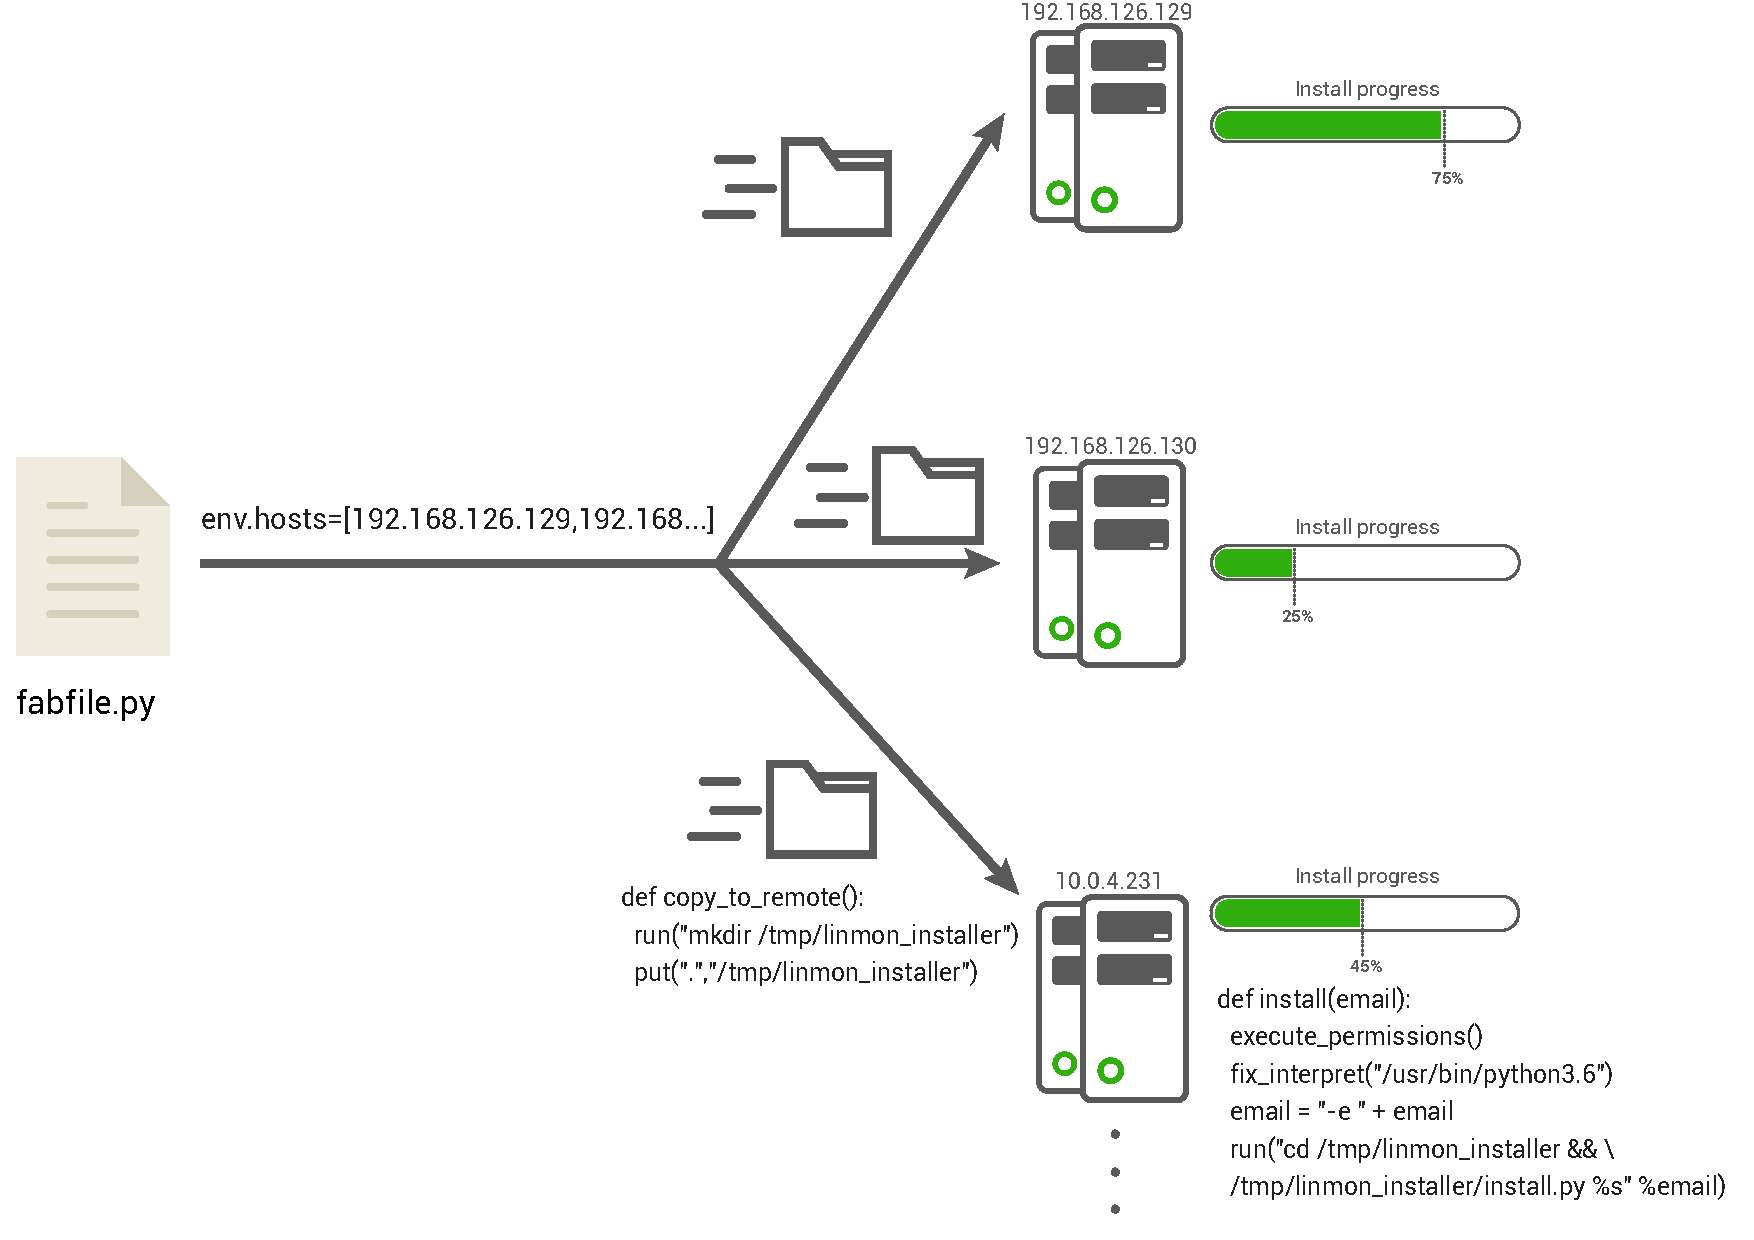
\includegraphics{obrazky-figures/fabric_pic.pdf}}
		\vspace{-1em}
		\caption{Schéma práce nasadzovacieho skriptu}
		\label{fabric_schema}
	\end{center}
\end{figure} 

\chapter{Testovanie}
\label{testovanie}
Táto kapitola sa venuje testovaniu či už nástroju ako celku, tak aj testovaniu jednotlivých vybraných kľúčových častí hlavného skriptu. V~neposlednom rade sa taktiež zaoberá testovaním filtrovania notifikačných správ, čo patrí k~nosným bodom celej tejto práce. Výsledky testovania jednotlivých monitorovacích modulov nie sú súčasťou tejto kapitoly, nakoľko boli testované počas implementácie a vzhľadom k~množstvu skriptov by rozsah tejto kapitoly značne znásobili. Po dôkladnom zvážení bolo vypustené testovanie užívateľského rozhrania nakoľko primárnymi používateľmi skriptov sú pokročilí užívatelia\,--\,systémoví administrátori, preto sa testovanie sústreďuje skôr na kľúčové prvky skriptov. 

\section{Testovacie prostredie}
Testovanie všetkých súčastí programu, teda hlavného skriptu a monitorovacích modulov prebiehalo v~dvoch typoch zariadení, a to na fyzickom a virtuálnom, jednotlivé testovacie prostredia môžeme vidieť v~tabuľkách \ref{phys_dev}, \ref{virt_dev1}, \ref{virt_dev2}, \ref{virt_dev3}. Ako si môžeme všimnúť, tak na jednotlivých testovacích strojoch boli nainštalované rôzne distribúcie GNU/Linux s~rôznymi init systémami, a to umožnilo otestovanie funkčnosti na \texttt{SystemD}, \texttt{SysV} a \texttt{Upstart}. Naviac bola otestovaná prenositeľnosť nástroju Linmon naprieč distribúciami založenými na RHEL a Debian. Pre skrátenie veľkosti tabuliek bola zo zoznamu odstránená absolútna cesta ku skriptom \texttt{/opt/linmon/monitoring\_scripts}.


Na fyzickom zariadení z~tabuľky \ref{phys_dev} boli testované prevažne monitorovacie moduly monitorujúce disky. Tento prístup bol zvolený z~dôvodu, že na virtuálnych zariadeniach nie je možné odčítať hodnoty S.M.A.R.T a taktiež teplotu virtuálnych diskov. Naviac bola pri monitorovaní zmenená IP adresa rozhrania a pripojený disk, ktorý nebol špecifikovaný ako povolený, čo malo za následok notifikáciu administrátora.
\\ 
\begin{table}[H]
	\catcode`\-=12
	\begin{center}
		\begin{tabular}{|l|l|}
			\hline
			\textbf{CPU} & Intel i5 6200 2 cores/ 4 threads  \\
			\hline
			\textbf{RAM} & 8192MB  \\
			\hline
			\textbf{HDD/SSD} & 500GB HDD NTFS, 256GB SSD (113GB EXT4) \\
			\hline
			\textbf{OS} & Debian 10 64bit, SystemD, Kernel 4.15.0 \\
			\hline
			\textbf{NET}& lo (loopback), enp0s31f6 (ethernet), wlp3s0 (Wi-Fi)\\
			\hline
			\multirow{8}{*}{\textbf{Linmon CRON}}  & 5 ./user\_cpu\_usage.py mysql -t 10 -i error\\
			& 5 [DISK] ./disk\_temp.py -a -t 30 -i warning\\
			& 5 [DISK] ./disk\_allow\_serial.py -i warning\\
			& 5 [AUTH] ./rsyslog\_auth.py -i critical\\
			& 10 [NETCARD] ./netcard\_ip\_change.py -i error\\
			& 15 [DISKUSE] ./disk\_usage.py -b /dev/sda1 -p 10 -i critical\\
			& 00:00 [SMART] ./disks\_smart\_mon.py -i critical\\
			& 60 [DISKUSE] ./disk\_usage.py -b /dev/sda1 -p 10 -i critical\\
			\hline			
		\end{tabular}
		\caption{Fyzický stroj}
		\label{phys_dev}
	\end{center}
\end{table}

Virtuálny stroj č.1 bol webový server, pri ktorom boli monitorované služby s~nim súvisiace, a to démon webserveru Apache a databázy Mysql. Boli vyvolané podmienky na notifikáciu pri vypnutí jednej z~týchto služieb, následne bola vyvolaná žiadosť o~prístup k~\texttt{/etc/passwd}, čo spôsobilo notifikáciu za pomoci skriptu \texttt{rsyslog\_apache.py}. Nakoniec bolo vypnuté virtuálne zariadenie s~IP adresou \texttt{192.168.126.131}, čo vyvolalo príslušnú notifikáciu.
\\
\begin{table}[H]
	\catcode`\-=12
	\begin{center}
		\begin{tabular}{|l|l|}
			\hline
			\textbf{CPU} & 2 cores \\
			\hline
			\textbf{RAM} & 2048MB  \\
			\hline
			\textbf{HDD/SSD} & 20GB vmdk EXT4 \\
			\hline
			\textbf{OS} & Centos 7 64bit, SystemD, Kernel 3.10.0 \\
			\hline
			\textbf{NET}& lo (loopback), ens33 (ethernet)\\
			\hline
			\multirow{7}{*}{\textbf{Linmon CRON}}  & 5 ./user\_cpu\_usage.py mysql -t 10 -i error\\
			& 5 [APACHE] ./proc\_ram\_mon.py apache -p 40 -i warning\\
			& 5 [APACHE] ./proc\_cpu\_mon.py apache -p 50 -i info\\
			& 5 [APACHE] ./rsyslog\_apache.py -i error\\
			& 2 [SERVICE] ./service\_alive\_stat.py -i critical -a httpd\\
			& 2 [SERVICE] ./service\_alive\_stat.py -i critical -a mysqld\\
			& 1 ./node\_alive.py -s 192.168.126.131 -t 4 -i critical\\
			\hline			
		\end{tabular}
		\caption{Virtuálny stroj 1}
		\label{virt_dev1}
	\end{center}
\end{table}

\newpage
Na virtuálnom stroji č.2 bolo monitorované vyťaženie hardvéru, pričom simulácia tohto vyťaženia bola realizovaná programom \texttt{stress}. Napokon boli monitorované služby \texttt{postfix}, \texttt{named} a \texttt{sendmail} a notifikácia bola vyvolaná ich zastavením. Tak ako v~predchádzajúcom virtuálnom stroji, tak aj v~tomto sa simulovalo vypnutie susedného zariadenia s~následnou notifikáciou o~jeho neaktívnosti.
\begin{table}[H]
	\catcode`\-=12
	\begin{center}
		\begin{tabular}{|l|l|}
			\hline
			\textbf{CPU} & 2 cores \\
			\hline
			\textbf{RAM} & 4096MB  \\
			\hline
			\textbf{HDD/SSD} & 20GB vmdk EXT4 \\
			\hline
			\textbf{OS} & Ubuntu 14.04 64bit, Upstart, Kernel 4.4.0 \\
			\hline
			\textbf{NET}& lo (loopback), eth0 (ethernet)\\
			\hline
			\multirow{7}{*}{\textbf{Linmon CRON}}  & 5 [RES] ./ram\_free\_mon.py -p 20 -i error\\
			& 5 [RES] ./cpu\_mon.py -t 80 -i critical\\
			& 5 [RES] ./swap\_mon.py -p 20 -i critical\\
			& 2 [SERVICE] ./service\_alive\_stat.py -i critical -a postfix\\
			& 2 [SERVICE] ./service\_alive\_stat.py -i critical -a sendmail\\
			& 2 [SERVICE] ./service\_alive\_stat.py -i critical -a named\\
			& 1 ./node\_alive.py -s 192.168.126.129 -t 4 -i warning\\
			\hline			
		\end{tabular}
		\caption{Virtuálny stroj 2}
		\label{virt_dev2}
	\end{center}
\end{table}

Na poslednom testovacom stroji č.3 bol podobne ako na predchádzajúcom monitorovaný hardvér a živosť ďalšieho susedného stroja. Naviac tento virtuálny stroj obsahoval softvérové RAID polia typu 0, 1 a 5, na ktorých boli zámerne vyvolané chyby s~cieľom otestovať notifikáciu pomocou emailu. Poslednou testovanou časťou bola notifikácia nových pripojených USB zariadení, ktoré by mohli byť v~reálnej prevádzke nechcené a obsahovať škodlivé kódy.

\begin{table}[H]
	\catcode`\-=12
	\begin{center}
		\begin{tabular}{|l|l|}
			\hline
			\textbf{CPU} & 2 cores \\
			\hline
			\textbf{RAM} & 4096MB  \\
			\hline
			\textbf{HDD/SSD} & 20GB vmdk EXT4 \\
			\hline
			\textbf{OS} & Devuan Jessie 1.0 64bit, SysV, Kernel 3.16.0 \\
			\hline
			\textbf{NET}& lo (loopback), eth0 (ethernet)\\
			\hline
			\multirow{8}{*}{\textbf{Linmon CRON}}  & 5 [RES] ./ram\_free\_mon.py -p 20 -i error\\
			& 5 [RES] ./cpu\_mon.py -t 80 -i critical\\
			& 5 [RES] ./swap\_mon.py -p 20 -i critical\\
			& 2 [SERVICE] ./service\_alive\_stat.py -i critical -a cupsd\\
			& 1 ./node\_alive.py -s 192.168.126.130 -t 4 -i warning\\
			& 10 [NEWDEVS] ./dev\_usb\_new.py -i info \\
			& 10 [NEWDEVS] ./disk\_allow\_uuid.py -i warning\\
			& 60 ./disk\_health\_mdadm -a -i error\\
			\hline			
		\end{tabular}
		\caption{Virtuálny stroj 3}
		\label{virt_dev3}
	\end{center}
\end{table}
\newpage
\section{Testovanie mechanizmu vysokej dostupnosti}
Ako už bolo spomenuté v~predchádzajúcich kapitolách, tak na zaistenie stáleho chodu programu sú použité dva od seba nezávislé prístupy. Prvým testovaným prístupom je reštartovanie služby pri výpadku za pomoci init systému. Na nižšie uvedenom výpise procesov môžeme vidieť bežiaci proces s~PID 372.

\begin{verbatim}
UID    PID   PPID C STIME TTY TIME     CMD
root   372   1    0 08:16 ?   00:00:00 /usr/bin/python3 /opt/linmon/linmon.py
\end{verbatim}

Na simuláciu výpadku bol zadaný príkaz \texttt{kill -9 372}, ktorý spôsobil zastavenie bežiaceho procesu. Bezodkladne po zastavení procesu sa monitorovací nástroj znovu spustí, čo dokazuje aj nasledovný výpis z~bežiacich procesov.
\begin{verbatim}
UID    PID   PPID C STIME TTY TIME     CMD
root   398   1    0 08:16 ?   00:00:00 /usr/bin/python3 /opt/linmon/linmon.py
\end{verbatim}

Druhý spôsob zaisťujúci nepretržitý beh, záznam v~plánovači \texttt{cron}, bude spustený len v~prípade zlyhania skriptu init systému, prípadne pokiaľ by predbehol proces reštartu init systémom.

\begin{verbatim}
UID    PID   PPID C STIME TTY TIME     CMD
root   639   1    0 08:29 ?   00:00:00 /usr/bin/python3 /opt/linmon/linmon.py
\end{verbatim}

Po spustení monitorovania má skript PID 639 a  po aplikovaní príkazu \texttt{kill -9 639} sa proces monitorovania skriptu zastaví. Následne záznam v~crone zabezpečí opätovné spustenie, čo môžeme vidieť na výpise nižšie. 

\begin{verbatim}
UID    PID   PPID C STIME TTY TIME     CMD
root   681   679  0 08:30 ?   00:00:00 /bin/sh -c /opt/linmon/linmon.py
root   682   681  4 08:30 ?   00:00:00 /usr/bin/python3 /opt/linmon/linmon.py

\end{verbatim}

\section{Filtrovanie notifikačných správ}
Testovanie filtrovania emailových správ prebiehalo na zariadení z~tabuľky \ref{phys_dev} pričom pre prijímanie správ bol použitý program Mozilla Thunderbird v. 52.5.2. Na obrázku \ref{thunderbird_filter_settings} je definované pravidlo pre filtrovanie správ, v~ktorých predmet obsahuje najnižšiu možnú úroveň závažnosti notifikácie, pričom pri prijatí správy so značkou \texttt{info} premiestni túto správu do separátneho priečinku. Priečinok s~vyfiltrovanými správami, ktoré obsahujú značku \texttt{info} môžeme vidieť na obrázku \ref{thunderbird}. Keďže predmet správy obsahuje ďalšie dôležité značky ako napríklad hostname, skupinu z~plánovača a oneskorenie spustenia skriptov, prípadne čas spustenia, tak je možné na základe všetkých týchto značiek logicky roztriediť notifikačné správy. Naviac je možné správy vyfiltrovať aj podľa parametrov monitorovaného zariadenia z~tela správy. Notifikačné správy je teda možné bez problémov organizovať či už podľa závažnosti správ, monitorovaných súčastí systému, frekvencie spúšťania skriptov a rôznych iných vlastností.
\\
\begin{figure}[H]
	\begin{center}
		\scalebox{0.4}{\includegraphics{obrazky-figures/thunderbird_settings_filter.png}}
		\vspace{-0.5em}
		\caption{Nastavenie filtrovania prijatých správ}
		\label{thunderbird_filter_settings}
	\end{center}
\end{figure} 
\vspace{-1.5em}
\begin{figure}[H]
	\begin{center}
		\scalebox{0.4}{\includegraphics{obrazky-figures/thunderbird.png}}
		\vspace{-0.5em}
		\caption{Vyfiltrované správy v~separátnom priečinku}
		\label{thunderbird}
	\end{center}
\end{figure} 
\section{Testovanie módu údržby}
Mód údržby slúži na pozastavenie monitorovania, preto je nutné otestovať jeho funkčnosť, a to predovšetkým notifikáciu o~začiatku a konci údržby a pozastavenie zasielania správ. Na nasledujúcom výpise z~prijatých správ môžeme vidieť, že o~9:01 bol aktivovaný mód údržby pomocou príkazu \texttt{./linmon.py -m on}.

\begin{verbatim}
Subject                                       Correspondent   Date
                                  .
                                  .
                                  .
LINMON[thinkpadl460][warning][5min][DEFAULT]  root            26.4.2018 8:41
LINMON[thinkpadl460][info][5min][RAM]         root            26.4.2018 8:41
LINMON[thinkpadl460][info][5min][RAM]         root            26.4.2018 8:46
LINMON[thinkpadl460][info][10min][NEWDEVICE]  root            26.4.2018 8:46
LINMON[thinkpadl460][info][5min][RAM]         root            26.4.2018 8:51
LINMON[thinkpadl460][error][15min][DISKUSE]   root            26.4.2018 8:51
LINMON[thinkpadl460] Maintenance mode ON      root            26.4.2018 9:01
\end{verbatim}

Mód údržby bol spustený po dobu 50 minút, kedy sa zadal príkaz na jeho vypnutie \texttt{./linmon.py -m off}, následne, ako môžeme vidieť na výpise nižšie, tak monitorovanie plynulo pokračovalo ďalej.

\begin{verbatim}
Subject                                       Correspondent   Date
                                  .
                                  .
                                  .
LINMON[thinkpadl460][error][15min][DISKUSE]   root            26.4.2018  8:51
LINMON[thinkpadl460] Maintenance mode ON      root            26.4.2018  9:01
LINMON[thinkpadl460] Maintenance mode OFF     root            26.4.2018  9:51
LINMON[thinkpadl460][warning][5min][DEFAULT]  root            26.4.2018  9:56
LINMON[thinkpadl460][info][5min][RAM]         root            26.4.2018  9:56
LINMON[thinkpadl460][info][5min][RAM]         root            26.4.2018 10:01
\end{verbatim}

\chapter{Záver}
Cieľom tejto bakalárskej práce bol návrh a následná implementácia monitorovacích skriptov, ktoré budú sledovať stav počítačových clusterov s~následnou notifikáciou systémových administrátorov. Implementačným jazykom bol skriptovací jazyk Python 3 pričom pri implementácií bol braný ohľad na minimálny počet programov, ktoré je nutné nainštalovať na zaistenie práce monitorovacieho nástroja. Z~tohoto dôvodu sú ako notifikačný prostriedok použité emailové správy, a teda jedinými dvoma nutnými programami pre chod hlavného monitorovacieho a notifikačného skriptu sú interpret jazyka Python 3.5 alebo vyšší a program \texttt{sendmail}.

Výsledný monitorovací program vylepšuje metódu monitorovania tým, že oproti štandardnému prístupu, kde sú v~plánovači \texttt{cron} zadané skripty na monitorovanie a každý skript posiela emailovú správu, umožňuje program Linmon zoskupovať výstupy viacerých skriptov do jednej správy a tým nezahlcovať emailovú schránku. Navyše umožňuje efektívne filtrovanie správ na základe značiek v~predmete správy. Oproti systémom akými sú Nagios a Zabbix nie je nutná inštalácia balíčkov pre hlavný monitorovací skript, nakoľko inštalácie v~niektorých proprietárnych systémoch môžu byť zakázané. Okrem vyššie spomenutých vlastností bol skript vyvíjaný s~ohľadom na prenositeľnosť naprieč rôznymi distribúciami, a to podporou init systémov \texttt{SystemD}, \texttt{SysV} a \texttt{Upstart} ako aj podporou rôznej hierarchie súborového systému. Taktiež umožňuje jednoduchú modifikáciu už existujúcich skriptov a tvorbu nových, čomu dopomáha ako návod, tak aj vzorové skripty.

Monitorovacie moduly umožňujú zisťovanie vysokých záťaží zdrojov zariadenia, monitorovanie záznamov syslog a monitorovanie služieb systému, ktoré poskytnú výstup hlavnému skriptu, ktorý môže zoskupiť viacero výstupov do jednej správy a následne notifikuje administrátora.

Kvôli implementácií bolo nutné naštudovať záznamy syslog rôznych známych a často používaných programov v~serverových systémoch GNU/Linux. Táto časť riešenia bakalárskej práce bola jednou z~najobtiažnejších, čo sa týka získavania informácií, nakoľko výstupy záznamov syslog nie sú jednoducho získateľné kvôli citlivým dátam. Z~tohto dôvodu bol počet skriptov monitorujúcich záznamy syslog o~niečo zmenšený oproti pôvodnému návrhu.

Do budúcnosti sa počíta s~rozšírením počtu skriptov monitorujúcich záznamy syslog a taktiež optimalizácií filtrovacích značiek umožňujúcich triedenie notifikačných emailov na základe reálneho používania. Ďalším možným rozšírením implementovaným v~budúcnosti bude pridanie podpory pre \texttt{journalctl}, ktorý sa používa v~distribúcii Fedora na prehliadanie záznamov syslog.





\nocite{*}

%=========================================================================
